\section{Grundlagen der statistischen Physik}
\subsection{Mikrozustand, Makrozustand, statistisches Ensemble}

\begin{definition}{Mikrozustand}
    Ein Zustand bei dem sämtliche Information über das System bekannt ist.
    \begin{itemize}
        \item qm: \ Zustand $\ket{\Psi}$, Vektor im Hilbert-Raum 
        \item klass.: \ Orte und Impulse aller Teilchen 
    \end{itemize}
\end{definition}

\begin{beispiel}{Beispiel}
    \begin{itemize}
    \item Elektron mit $z^+$ Spin (vgl. Stern-Gerlach-Experiment)
    \item Grundzustand im \textbf{HO} (Harmonischen Oszillator)
    \item Superposition von 2. + 3. angeregten Zustand: $ \frac{1}{\sqrt{2}}(\ket{2} + \ket{3})$
    \item System von 100 Spins: $\underbrace{\text{1. Spin } z^+\text{, 2.Spin } x^-, \dots, \text{ 100. Spin } y^+}_{\text{Superpositionen}}$
 \end{itemize}
\end{beispiel}



\begin{definition}{Makrozustand}
    Das System wird durch makroskopische Größen (Gesamtenergie, Magnetisierung, Entropie) beschrieben, wobei die Details über den zugrundeliegenden Mikrozustand unbekannt sind und dieser auch \textbf{nicht messbar} ist (meist auch nicht nötig). Viele Mikrozustände führen zu dem gleichen Makrozustand. Es ist aber möglich, statistische Aussagen über den Mikrozustand zu treffen.
\end{definition}

\begin{beispiel}{Beispiel statistische Aussage:}
Zustand $\ket{\Psi}$ mit \textbf{WS} (Wahrscheinlichkeit) $w_m$, wobei gilt: $\forall m: w_m \geq 0 \wedge \sum_m w_m = 1 \quad (\Rightarrow \forall m: w_m \leq 1)$
\end{beispiel}
 
\begin{definition}{Statistisches Ensemble}
    Man denkt sich eine große Menge von Kopien des Systems, die alle den gleichen Makrozustand haben. Jede dieser Kopien ist in einem Mikrozustand $\ket{\Psi_n}$ mit WS $w_n$.\\ $\Rightarrow$ wesentlich mehr Kopien als Anzahl Mikrozustände
\end{definition}

\subsection*{Ziel der statistischen Physik}
\begin{itemize}
    \item Theorie für WS $w_n$
    \item basierend auf \glqq sinnvollen\grqq \, Annahmen
    \item experimentelle Aussagen
\end{itemize}


\subsection{Dichteoperator (statistischer Operator)}     \marginpar{VL 2}

Wie beschreibt man einen Makrozustand / statistisches Ensemble?

\vspace{0.5cm}
\underline{Idee}
\begin{itemize}
    \item [$\rightarrow$] Superposition: $\sum_n w_n \ket{\Psi_n}$ \textbf{nicht richtig}: immer noch Mikrozustand, nur normiert für $w_n \rightarrow \sqrt{w_n}$, falsche Aussagen für Messungen
\end{itemize}

\begin{beispiel}{Beispiel: polarisiertes Licht}
    \begin{itemize}
    \item Makrozustand: 50 \% $\updownarrow$, 50 \% $\leftrightarrow$
    \item Messung mit $\nearrow$ Polarisator: 50 \% Intensität (jede Polarisationsrichtung lässt 50 \% Intensität durch (2 * 0.5 * 50 \% = 50 \%)
    \item falsche Beschreibung: Superposition: $\frac{1}{\sqrt{2}} ( \ket{\updownarrow} + \ket{\leftrightarrow}) = \ket{\nearrow}$
    \item[$\Rightarrow$] 100 \% Intensität
\end{itemize}
\end{beispiel}



\begin{definition}{Dichteoperator}
    \begin{equation}
        \hat{\varrho} := \sum_n w_n \ket{\Psi_n} \bra{\Psi_n}
    \end{equation}

    \begin{itemize}
        \item $\ket{\Psi_n}$ müssen normiert sein: $\bra{\Psi_n}\ket{\Psi_n} = 1$
        \item $\ket{\Psi_n}$ müssen nicht orthogonal sein (z.B.: 20\% $\updownarrow$, 80\% $\leftrightarrow$)
        \item $\sum_n \rightarrow \int dn$ , falls kontinuierlich
    \end{itemize}
\end{definition}

$\ket{\Psi_n}\bra{\Psi_n}$ ist \underline{Projektionsoperator}
\begin{definition}{Projektionsoperator}
\begin{equation}
    P^2 = P
\end{equation}
\end{definition}



\begin{proof}
\begin{equation}
    \ket{\Psi}\underbrace{\bra{\Psi}\ket{\Psi}}_{=1}\bra{\Psi} = \ket{\Psi}\bra{\Psi}
\end{equation}
$\ket{\Psi}\bra{\Psi}$ ist Projektionsoperator.

\end{proof}

$P = \ket{\Psi}\bra{\Psi}$ projiziert auf Zustand $\ket{\Psi}$

\begin{proof}
    \begin{equation}
        P \ket{\varphi} = \ket{\Psi} \bra{\Psi} \ket{\varphi} = \bra{\Psi}\ket{\varphi}\ket{\Psi} \ \  \parallel \ket{\Psi}
    \end{equation}
\end{proof}

\subsubsection{Reine Zustände}
 System sei in normierten Zustand $\ket{\Psi}$ ($\bra{\Psi}\ket{\Psi} = 1$). Ziel: Vorhersagen für Messung einer Observablen $A$:
 \begin{itemize}
     \item Eigenwertgleichung zu selbstadjunggierten\footnote{In der Vorlesung wird diese Eigenschaft anscheinend fälschlicher Weise als "hermitesch" bezeichnet.} Operator $A$: \ \ $A^{\dag} = A$
     \begin{equation}
         A \ket{\alpha_k} = a_k \ket{\alpha_k}
     \end{equation}
     \item Eigenwerte $a_k$ sind mögliche Messergebnisse
     \item Eigenzustände $\ket{\alpha_k}$
    \begin{itemize}
         \item[-] orthonormiert: $\bra{\alpha_l}\ket{\alpha_k} = \delta_{l,k}$
         \item[-] vollständig: $\sum_k \ket{\alpha_k}\bra{\alpha_k} = \mathds{1}$ \makebox(0,0){\put(0,2.2\normalbaselineskip){%
               $\left.\rule{0pt}{1.1\normalbaselineskip}\right\}$ $\{ \ket{\alpha_k}\}$ ist VONS}}
     \end{itemize}
     \item Zustand $\ket{\Psi}$ entwickeln in $\ket{\alpha_k}$:
         \begin{equation}
             \ket{\Psi} = \sum_k c_k \ket{\alpha_k} \ \ \ \text{mit} \ c_k = \bra{\alpha_k}\ket{\Psi}
         \end{equation}
    \begin{proof}
        \begin{equation}
            \ket{\Psi} = \underbrace{\sum_k \ket{\alpha_k}\bra{\alpha_k}}_{= \mathds{1}} \ket{\Psi} = \ket{\Psi}
        \end{equation}
    \end{proof}
    \item Messung von $A$ ergibt Eigenwert $a_k$ mit WS $p_k = \left|c_k \right| ^2 = \left| \bra{\alpha_k}\ket{\Psi}\right|^2$ (\emph{Born'sche Regel})
    \begin{proof}
        \begin{equation}
            \sum_k p_k = \sum_k \braket{\Psi}{\alpha_k}\braket{\alpha_k}{\Psi} = \bra{\Psi}\underbrace{\sum_k \ket{\alpha_k}\bra{\alpha_k}}_{= \mathds{1}} \ket{\Psi} = \braket{\Psi}{\Psi} = \mathds{1}
        \end{equation}
    \end{proof}
    \item \underline{Erwartungswert} von $A$ für Zustand $\ket{\Psi}$:
    \begin{equation}
        \langle A \rangle := \bra{\Psi}A\ket{\Psi} = \sum_k \bra{\Psi}A\ket{c_k \alpha_k} = \sum_k c_k a_k \underbrace{\braket{\Psi}{\alpha_k}}_{c_k^*} = \sum_k \left| c_k \right|^2 a_k = \sum_k p_k a_k
    \end{equation}

 \end{itemize}
 
Die WS $p_k$ sind rein qm Natur. Mit ihnen kann man die WS für Messergebnisse $a_k$ vorhersagen.

\textbf{Achtung: falsche Aussage:} \glqq System ist mit WS $p_k$ im Zustand $\ket{a_k}$ \grqq $\rightarrow$ System kollabiert bei Messung in Eigenzustand (vgl. QM I)

\subsubsection*{Dichteoperator}
äquivalentes Konzept für reinen Zustand $\ket{\Psi}$, $\hat{\varrho} = \ket{\Psi} \bra{\Psi}$

\begin{equation}
    \Rightarrow p_k = |\braket{a_k}{\Psi}|^2 = \braket{a_k}{\Psi}\braket{\Psi}{a_k} = \bra{a_k} \hat{\varrho} \ket{a_k}
\end{equation}
\begin{align}
    \langle A \rangle = \bra{\Psi} A \ket{\Psi} = \sum_k c_k \bra{\Psi} A \ket{a_k} = \sum_k \braket{a_k}{\Psi} \bra{\Psi} A \ket{a_k} = \underbrace{\sum_k \bra{a_k} \hat{\varrho} A \ket{a_k}
    = \trace \hat{\varrho} A}_{\text{da $\ket{a_k}$ VONS}}
\end{align}

\underline{Vorteile des Dichteoperators (reine Zustände):}
\begin{itemize}
    \item beliebiger Phasenfaktor in $\ket{\Psi}$, aber nicht in $\hat{\varrho} = \ket{\Psi} \bra{\Psi}$
    \item $\langle A \rangle$ ist linear in $\hat{\varrho}$, aber quadratisch in $\ket{\Psi}$
\end{itemize}

\subsubsection*{Eigenschaften der Spur}
\begin{definition}{Spur}
    \begin{equation}
        \trace X := \sum_n \bra{\varphi_n}X\ket{\varphi_n} \ \ \ \text{ mit bel. VONS } \{\ket{\varphi_n}\} \text{ (von Basis unabhängig)}
    \end{equation}
    \begin{align}
        \trace (X+Y) &= \trace X + \trace Y  \\ 
        \trace(cX) &= c \cdot \trace X  \ \ c \in \mathbb{C} \\
        \trace (XY) &= \trace(YX) \   \Rightarrow \ \trace(XYZ) = \trace(YZX) = \trace (ZXY) \text{ zyklisch!} \\
        \trace (X^{\dag}) &= (\trace X)^* \\
        \trace(\ket{\varphi}\bra{\Psi}) &= \braket{\Psi}{\varphi}
    \end{align}
\end{definition}

\subsubsection{gemischte Zustände}
Makrozustand (Ensemble) vieler möglicher Mikrozustände $\ket{\Psi_n}$ mit WS $w_n$ ($w_n \geq 0, \sum_n w_n = 1, \ket{\Psi_n} \text{ normiert, i.A. nicht orthogonal})$

$\rightarrow$ alle Informationen aus Dichteoperator bestimmbar:
\begin{itemize}
    \item WS für Messergebnis $a_k$:
    \begin{align}
        p_k &= \sum_n w_n |\braket{a_k}{\Psi_n}|^2 \quad \text{\glqq Mitteln über Mikrozustände \grqq} \\
        &= \sum_n w_n\bra{a_k} \ket{\Psi_n} \bra{\Psi_n} \ket{a_k} \\
        &= \bra{\alpha_k} \underbrace{\sum_n w_n \ket{\Psi_n}\bra{\Psi_n}}_{=\varrho} \ket{\alpha_k} = \bra{a_k} \hat{\varrho} \ket{a_k}
    \end{align}
    \item Erwartungswert von A:
    \begin{align}
        \langle A \rangle &= \sum_n w_n \underbrace{\bra{\Psi_n} A \ket{\Psi_n}}_{\trace () \text{, da nur komplexe Zahl}} \\
        &= \sum_n w_n \trace(\ket{\Psi_n} \bra{\Psi_n} A )\\
        &= \trace \bigl(\sum_n w_n \ket{\Psi_n} \bra{\Psi_n} A \bigr) = \trace( \hat{\varrho} A)
    \end{align}

    \begin{equation}
        \fcolorbox{red}{white}{$\langle A \rangle = \trace( \hat{\varrho} A)$}
    \end{equation}
\end{itemize}

Verschiedene $\{ \ket{\Psi_n}, w_n \}$ können zu gleichen $\varrho$ führen.
Sie beschreiben den gleichen Makrozustand.
Kein Experiment kann (im Rahmen der Quantenmechanik) einen Unterschied finden!


\begin{prop}{Eigenschaften von $\varrho$}
 \begin{equation*}
     \begin{rcases*}
        &\qq{1.}  $\varrho^{\dag} = \varrho \ $ selbstadjungiert\footnote{laut Ketzmerick "hermitesch"}\\
        &\qq{2.} $\trace \varrho = 1$ \\
        &\qq{3.} \text{Positivität } \forall \ket{\varphi}: \; \bra{\varphi} \varrho \ket{\varphi} \geq 0 \;\\
        &\qquad \Leftrightarrow \text{ alle Eigenwerte } \geq 0
    \end{rcases*} \Leftrightarrow \varrho \quad \text{ist Dichteoperator} 
 \end{equation*}
\end{prop} 

\newpage
 \subsubsection*{Unterschiede zwischen reinen und gemischten Zuständen}
\begin{multicols}{2}
 \underline{reiner Zustand}
 \begin{itemize}
     \item $\varrho ^2 = \varrho$
     \begin{proof}
         $\varrho ^2 = \ket{\Psi} \underbrace{\braket{\Psi}}_{\mathds{1}} \bra{\Psi} = \varrho$
     \end{proof}
     \item $\trace \varrho^2 =1$
 \end{itemize}
 \columnbreak
 \underline{gemischter Zustand (nicht reiner Zustand)}
 \begin{itemize}
     \item $\varrho ^2 \neq \varrho$
     \item $\trace\varrho^2 < 1$
     \item[] 
     \item[]
 \end{itemize}
\end{multicols}
\subsubsection{Dichtematrix}

\begin{definition}{Dichtematrix in bel. VONS $\{ \ket{\Phi_k}\}$}
    \begin{equation}
        \varrho_{lk} := \bra{\Phi_k} \hat{\varrho} \ket{\Phi_l}
    \end{equation}
    
\end{definition}

\begin{itemize}     \marginpar{VL 3}
    \item Kenntnis aller Matrixelemente enthält volle Information
    \item wähle als Basis $\{\ket{\alpha_k}\}$ (Eigenzustände der Observablen A: \ $A \ket{\alpha_k} = a_k \ket{\alpha_k}$)
    \item [$\Rightarrow$] physikalische Bedeutung
    \begin{itemize}
        \item Diagonalelemente $\varrho_{kk} = \bra{\alpha_k} \varrho \ket{\alpha_k} \stackrel{s.o.}{=} p_k \geq 0$ (Besetzung)\\
        Dies ist die Wahrscheinlichkeit, $a_k$ zu messen.
        \item $\varrho_{kk} = p_k$ enthält zwei Wahrscheinlichkeitsaussagen:
        \begin{enumerate}
            \item die quantenmechanische für reine Zustände (vgl. \emph{Born'sche Regel})
            \item die statistische aufgrund unvollständiger Information über das System 
        \end{enumerate}
        \item Nicht-Diagonalelemente $\varrho_{kl}$:  $\varrho_{kl} = \bra{\alpha_k} \varrho \ket{\alpha_l} = \sum_n w_n \bra{\alpha_k}\ket{\Psi_n}\bra{\Psi_n}\ket{\alpha_l}$ (Kohärenz [gibt Aussage über Phasenbeziehungen])
    \end{itemize}
\end{itemize}

\begin{beispiel}{Teilchen im Potential (H.O:) mit Eigenzuständen $\ket{n}$:}
$H\ket{n} = E_n \ket{n}$
\begin{itemize}
    \item[a)] reiner Zustand: 
    \begin{align}
        \ket{\Psi} &= \frac{1}{\sqrt{2}} \left( \ket{0} + \ket{1} \right) \\
        \Hat{\varrho} &= \ket{\Psi}\bra{\Psi} = \left( \frac{1}{\sqrt{2}} ( \ket{0} + \ket{1}) \right) \left(\frac{1}{\sqrt{2}} ( \bra{0} + \bra{1}) \right) \\
        &= \frac{1}{2}(\ket{0}\bra{0} + \ket{0}\bra{1} + \ket{1}\bra{0} + \ket{1}\bra{1})
    \end{align}
    \item[] Dichtematrix in der Basis $\{ \ket{n} \}$:
    \begin{equation}
        (\varrho)_{\{ \ket{n} \}} = (\varrho) = \begin{pmatrix}
            \frac{1}{2} & \frac{1}{2} & 0 & 0 & \dots \\
            \frac{1}{2} & \frac{1}{2} & 0 & 0 & \dots \\
            0 & 0 & 0 & 0 & \dots \\
            \vdots & \vdots & \vdots & \vdots & \ddots
            \end{pmatrix}
    \end{equation}
    \item[b)] gemischter Zustand: mit WS $\frac{1}{2}$ in $\ket{0}$ und mit WS $\frac{1}{2}$ in $\ket{1}$
    \begin{align}
        \varrho &= \frac{1}{2} \ket{0}\bra{0} + \frac{1}{2} \ket{1}\bra{1}
    \end{align}
    \item[] Dichtematrix in der Basis $\{ \ket{n} \}$:
    \begin{equation}
        (\varrho)_{\{ \ket{n} \}} = (\varrho) = \begin{pmatrix}
            \frac{1}{2} & 0 & 0 & 0 & \dots \\
            0 & \frac{1}{2} & 0 & 0 & \dots \\
            0 & 0 & 0 & 0 & \dots \\
            \vdots & \vdots & \vdots & \vdots & \ddots
        \end{pmatrix}
    \end{equation}
\end{itemize}
\end{beispiel}





$\Longrightarrow$ \textbf{Wie unterscheiden sich a) und b) bei der Messung?}

\subsubsection{Messung}
\begin{itemize}
    \item[] Observable A mit $A \ket{\alpha_k} = a_k \ket{\alpha_k}$
    \item[] Projektor\footnote{Projektoren haben immer Eigenwerte 0 und 1.} auf Zustand $\ket{\alpha_k}$: $P_k = \ket{\alpha_k}\bra{\alpha_k}$
    \item[] WS $a_k$ zu messen:
    \begin{equation*}
        p_k = \trace(P_k \varrho) = \sum_l \underbrace{\bra{\alpha_l}\ket{\alpha_k}}_{\delta_{kl}} \bra{\alpha_k} \varrho \ket{\alpha_l} = \bra{\alpha_k} \varrho \ket{\alpha_k} = \varrho_{kk}
    \end{equation*}
\end{itemize}

Dichteoperator nach Messung von $a_k$:
\begin{equation}
    \hat{\varrho}' = \frac{P_k \varrho P_k}{\trace(P_k \varrho P_k)} = \frac{P_k \varrho P_k}{\trace(P_k P_k \varrho)} = \frac{P_k \varrho P_k}{p_k} = \frac{\ket{\alpha_k} \bra{\alpha_k} \varrho \ket{\alpha_k} \bra{\alpha_k}}{\bra{\alpha_k} \varrho \ket{\alpha_k}} = \ket{\alpha_k} \bra{\alpha_k}
\end{equation}
$\Longrightarrow$ entspricht Postulat der QM zur Messung\\

Reiner Zustand: 
\begin{itemize}
    \item unabhängig von $\varrho$
    \item abhängig von A und Messergebnis
\end{itemize}

\subsubsection*{Vergleich Beispiele a) und b)\footnote{\textbf{Tangente aus Kais Übung:} \\ a) ist ist quantemnechanische Superposition wie bei Schödingers Katze: Katze ist gleichzeitig im Zustand lebendig und im Zustand tod.\\ b) klassischer Fall: entweder ein ZUstand oder der andere. \\ Unterschied zwischen klassischer Unsicherheit und quantenmechanischen Superposition steckt in Nebendiagonalen. \\Wie kommt man von quantenmechanischer Superposition zu klassischem Gemisch, das wir im ALltag beobachten? Antwort gibt die Theorie der offenen Quantensysteme (Betrachtung der Umgebung- Einfluss der Dekohärenz zerstören Nebendiagonalen). \\
Wie bereits bekannt können verschiedene Mikrozustände zum gleichen Dichteoperator führen (Siehe Blatt 2): \\ Intuition: Dichteoperator zeigt auch nichti}}
\begin{itemize}
    \item Messung Energie mit H: $H \ket{n} = E_n \ket{n}$ z.B. $ n = 0$
    \begin{equation}
        p_0 = \bra{0} \varrho \ket{0} = \varrho_{00} = \begin{cases}
            \frac{1}{2} & \text{, in a)} \\
            \frac{1}{2} & \text{, in b)}
        \end{cases}
    \end{equation}
    \item[$\rightarrow$] gleich, da Diagonale der Dichtematrix zur Basis $\{\ket{n}\}$ gleich
    \item Messung Ort mit X: $X \ket{x} = x \ket{x}$
    \item[] Ortsaufenthaltswahrscheinlichkeitsdichte (OAWD) $\downarrow$  
    \begin{equation}
         p(x) = \bra{x} \varrho \ket{x} = \begin{cases}
            \frac{1}{2}(|\varphi_0(x)|^2 + |\varphi_1(x)|^2 + 2 \Re{\varphi_0(x) \varphi_1^*(x)}) & \text{, in a)} \\
             \frac{1}{2}(\underbrace{\underbrace{ \bra{x} \ket{0}}_{\varphi_0(x)} \underbrace{\bra{0} \ket{x}}_{\varphi_0^*(x)}}_{|\varphi_0(x)|^2} + \underbrace{\bra{x} \ket{1} \bra{1} \ket{x}}_{|\varphi_1(x)|^2}) & \text{, in b)}
         \end{cases}
    \end{equation}
    \item[$\Rightarrow$] verschiedene Ergebnisse
\end{itemize}

\subsubsection{Zeitentwicklung}
\textbf{Frage:}
\begin{center}
    Wie sieht die Zeitentwicklung eines Makrozustands (durch Dichteoperator beschrieben) aus?
\end{center}


\begin{equation}
    \varrho(t) = \sum_n \underbrace{w_n(t)}_{\downarrow} \ket{\Psi_n(t)} \bra{\Psi_n(t)} 
\end{equation}

\begin{center}
    \small
    im abgeschlossenen System ändert sich die WS $w_n$ für Mikrozustand $\ket{\Psi_n(t)}$ nicht. \footnote{\textbf{Frage aus Plenum:} Warum sind die Wahrscheinlichketiten $w_n$ für abgeschlossene Systeme konstant? \\
    AW: Für abgeschlossene Systeme steckt die gesamte Zeitabhängigkeit in den $\ket{\Psi (t)}$. Gibt es eine Kopplung an die Umwelt, so steckt die Information für die Zeitabhängigkeit nur für Teilsysteme in den $\ket{\Psi (t)}$.}
\end{center}

\vspace{0.5cm}
Zeitentwicklung des Mikrozustandes:
\begin{align}
    \text{Schrödinger-GL: } i \hbar \frac{d}{dt} \ket{\Psi_n(t)} &= H(t) \ket{\Psi_n(t)} \\
    \text{adj. Gl: } - i \hbar  \frac{d}{dt} \bra{\Psi_n(t)} &=  \bra{\Psi_n(t)} \underbrace{H^{\dag}(t)}_{H^{\dag} = H}
\end{align}

\begin{enumerate}
\item DGL für Dichteoperator
\begin{align}
    \frac{d}{dt} \varrho (t) &= \sum_n w_n \left(\frac{d}{dt} \ket{\Psi_n(t)} \right) \bra{\Psi_n(t)} + \sum_n w_n \ket{\Psi_n(t)} \left(\frac{d}{dt} \bra{\Psi_n(t)} \right)\\
    &= \frac{1}{i \hbar} \left(\sum_n w_n H(t) \ket{\Psi_n(t)}\bra{\Psi_n(t)} - \sum_n w_n \ket{\Psi_n(t)}\bra{\Psi_n(t)} H(t) \right) \\
    &= \frac{1}{i \hbar} ( H(t) \varrho(t) - \varrho(t) H(t)) \\
    &= \frac{1}{i \hbar} [H(t), \varrho(t)] 
\end{align}

\vspace{0.5cm}
\item[$\Rightarrow$] \textbf{von-Neumann-Gleichung:}
\begin{equation}\label{Neumann}
    \fcolorbox{red}{white}{$\frac{d}{dt} \varrho (t) = \frac{1}{ih} [H(t), \varrho(t)]$}
\end{equation}
\vspace{0.5cm}

\item DGL für Dichtematrix (H sei zeitunabhängig): wähle ausgezeichnete Basis $\{\ket{k}\}$ der Eigenzustände von H:
\begin{align}
    H \ket{k} &= E_k \ket{k} \\
    \bra{k} H &= \bra{k} E_k
\end{align}

Matrixelemente der Dichtematrix in dieser Basis:
\begin{equation}
    \varrho_{kl}(t) = \bra{k} \varrho(t) \ket{l}
\end{equation}

Betrachte nun Zeitentwicklung:
\begin{align}
    \frac{d}{dt} \varrho_{kl}(t) &= \frac{1}{i \hbar}(\bra{k}H \varrho(t) \ket{l} - \bra{k} \varrho(t) \underbrace{H \ket{l}}_{E_l \ket{l}} \\
    &= \frac{1}{i \hbar} \bigl(E_k \varrho_{kl}(t) - E_l \varrho_{kl}(t) \bigr)
\end{align}

\begin{equation}   
    \Rightarrow \fcolorbox{red}{white}{$\frac{d}{dt} \varrho_{kl}(t) = \frac{E_k-E_l}{i \hbar} \varrho_{kl}(t)$}
\end{equation}


\end{enumerate}

\begin{prop}{Eigenschaften der Dichtematrix (zeitentwickelt)}
  \begin{enumerate}
    \item Diagonalelemente: $\frac{d}{dt} \varrho_{kk}(t) = 0 \Rightarrow \varrho_{kk}(t) = const. \quad \Rightarrow$  Besetzung $\varrho_{kk}$ von Energiezustand $\ket{k}$ konstant
    \item Nicht-Diagonalelemente: $\varrho_{kl}(t) = e^{- \frac{i}{\hbar}(E_k - E_l) t} \varrho_{kl}(0)$
    \begin{itemize}
        \item[$\Rightarrow$] Kohärenz $\varrho_{kl}$: Betrag konstant, Phase zeitabhängig
    \end{itemize}
\end{enumerate}  
\end{prop}


\subsubsection{Teilsysteme}
Gesamtsystem in reinem Zustand $\not\Longrightarrow$ Teilsystem durch reinen Zustand beschreibbar

\begin{beispiel}{reiner Zustand $\frac{1}{\sqrt{2}} \bigl(\ket{+ +} + \ket{- -} \bigr)$}
    \begin{equation*}
        \varrho = \frac{1}{2} \bigl( \ket{++}\bra{++} + \ket{++}\bra{--} +\ket{--}\bra{++} \ket{--}\bra{--}\bigr)    
        \end{equation*}
    Dichteoperator für Teilsystem 1. Spin: 
    \begin{equation*}
        \varrho_1 \overset{\text{\tiny{Spur über}}}{\underset{\text{\tiny{2. System bilden}}}{=}} \trace_2\varrho = \frac{1}{2}\bigl( \ket{+}\bra{+}+ \ket{-}\bra{-}\bigr) = \text{ Gemisch!}
    \end{equation*}
\end{beispiel}

\begin{itemize}
    \item Kein System ist wirklich abgeschlossen $\Rightarrow \ \exists$ Kopplung an Umgebung
    \begin{itemize}
         \item[$\Rightarrow$]jedes System ist eigentlich Teilsystem
    \end{itemize}
    \item Makroskopische Systeme haben exponentiell viele Mikrozustände
    \begin{itemize}
    \item[$\Rightarrow$] exponentiell kleine Energieabstände
    \item[$\Rightarrow$] auch kleine Kopplung an Umgebung ist groß gegenüber Energieabstände
    \item[$\Rightarrow$] makroskopische System = Teilsystem des Gesamtsystems inkl. Umgebung
    \item[$\Rightarrow$] Makrozustand = Gemisch $\rightarrow$ mit Dichteoperator beschreibbar
    \end{itemize}
\end{itemize}


\subsection{\glqq Dichteoperator\grqq{} in der klassischen Mechanik}     \marginpar{VL 4}
klassisches System mit $f$ Freiheitsgraden

\begin{itemize}
    \item[] \textbf{Mikrozustand:} $(q_1,\dots,q_f,p_1,\dots,p_f)=(\Vec{q}, \Vec{p})$
    \item[] Phasenraum: Raum aller $(\Vec{q}, \Vec{p})$, $2f$ Dimensionen
    \begin{itemize}
        \item[] \emph{Beispiel:} N Teilchen im 3D-Raum
        \item[$\rightarrow$] $f = 3 \cdot N$, Phasenraum: $6N$-Dimensional
        \item[] Mikrozustand ist Punkt im Phasenraum 
    \end{itemize}
    \item[] \textbf{Makrozustand:} Wahrscheinlichkeitsdichte $\varrho(\Vec{q}, \Vec{p})$ im Phasenraum
    \begin{itemize}
        \item[$\rightarrow$] \glqq Integral über viele Mikrozustände\grqq
    \end{itemize}
\end{itemize}

\begin{prop}{Eigenschaften von $\varrho$}
    \begin{itemize}
        \item Normierung:
        \begin{equation}
            \int \ \varrho(\Vec{q}, \Vec{p}) \ d\Vec{q} \ d\Vec{p} \ = \ 1 \qquad \text{QM: } \trace(\hat{\varrho}) = 1
        \end{equation}
        \item Positivität\footnote{Tatsächlich hat der quantenmechanische Dichteoperator die definierenden Eigenschaften Normierung, Positivität und der Selbstadjungiertheit. Letztere Eigenschaft besitzt kein sauberes klassisches Analogon. Man kann argumentieren, dass ein selbstadjungierter Operator reelle Eigenwerte besitzt und die klassische Wahrscheinlichkeitsdichte ebenfalls eine reelle Größe ist. (Eher schwammig, da eine rein komplexe Wahrscheinlichkeit nicht sinnvoll ist.)}:
        \begin{equation}
            \varrho(\Vec{q}, \Vec{p}) \geq 0 \qquad \text{QM: } \forall \ket{\Psi}: \bra{\Psi} \hat{\varrho} \ket{\Psi} \geq 0
        \end{equation}
        \item Erwartungswert von $A(\Vec{q}, \Vec{p})$:
        \begin{equation}
            \langle A \rangle = \int \ A \ \varrho(\Vec{q}, \Vec{p}) \ d\Vec{q} \ d\Vec{p} \qquad \text{QM: } \langle A \rangle = \trace(\varrho A) 
        \end{equation}
    \end{itemize}
\end{prop}

\subsubsection*{Zeitentwicklung}
\begin{itemize}
    \item Zeitentwicklung der Phasenraumtrajektorie $(\Vec{q}, \Vec{p})$ unter Hamiltonfunktion $H(\Vec{q}, \Vec{p})$ mittels Hamiltonschen Bewegungsgleichungen
    \begin{equation}\label{Hamilton}
        \dot{q}_i \ = \ \frac{\partial H}{\partial p_i} \qquad \dot{p}_i \ = \ -\frac{\partial H}{\partial q_i}
    \end{equation}
    \item \textbf{Liouville-Theorem:} Volumen eines zeitentwickelten Gebietes im Phasenraum bleibt erhalten
    \item Zeitentwicklung der Wahrscheinlichkeitsdichte $\varrho(\Vec{q}, \Vec{p}, t)$ entlang einer Phasenraumtrajektorie $(\Vec{q}, \Vec{p})$:
    \begin{equation}\label{Liouville}
        \frac{d}{dt} \varrho(\Vec{q}, \Vec{p}, t) \ = \ \frac{\partial \varrho}{\partial t} + \sum_i \left( \frac{\partial \varrho}{\partial q_i} \Dot{q}_i + \frac{\partial \varrho}{\partial p_i} \Dot{p}_i \right) \ = \ 0
    \end{equation}
    \item[] \centering{\textbf{Liouville-Gleichung}}
    \item Zeitentwicklung der Wahrscheinlichkeitsdichte $\varrho(\Vec{q}, \Vec{p}, t)$ am festen Phasenraumpunkt $(\Vec{q}, \Vec{p})$:
    \begin{equation}
        \frac{\partial \varrho}{\partial t} \overset{\equa{Hamilton}}{\underset{\equa{Liouville}}{=}} \sum_{i=1}^f \left( \frac{\partial \varrho}{\partial q_i} \frac{\partial H}{\partial p_i} - \frac{\partial \varrho}{\partial p_i} \frac{\partial H}{\partial q_i} \right) \ = \ - \underbrace{\{ \varrho, H\}}_{\text{Poisson-Klammer}}
    \end{equation}
    \begin{equation}
        \Longrightarrow \quad \frac{\partial \varrho}{\partial t} \ = \ \{ H, \varrho\} \quad \text{(entspricht Liouville-Gleichung)}
    \end{equation}
    \begin{equation}
        \text{QM: } \frac{d}{dt} \hat{\varrho}(t) \ = \ \frac{1}{i \hbar} [\hat{H}(t), \hat{\varrho}(t)] \quad \text{(von-Neumann-GL)}
    \end{equation}
\end{itemize}
\begin{itemize}
    \item Thermodynamisches Gleichgewicht
    \item[] $\quad$ Vorraussetzung: $H$ zeitunabhängig
    \begin{equation}
        \rightarrow \frac{\partial \varrho}{\partial t} \ = \ 0 \quad \Leftrightarrow \quad \{H,\varrho\}=0 \quad \overset{\varrho \text{ ist Fkt von H}}{\Longrightarrow} \quad \varrho = \varrho(H)
    \end{equation}
    \item[] \centering \emph{\glqq alle Orte mit gleichen $H$ haben gleiches $\varrho$\grqq} 
    \item[] QM: siehe unten
\end{itemize}


\subsection{Thermodynamisches Gleichgewicht}
Voraussetzung: zeitunabängiges System: $H \ket{n} \ = \ E_n \ket{n}$
\begin{itemize}
    \item[] Behauptung: \emph{Makroskopisches System strebt gegen thermodynamisches Gleichgewicht\footnote{dynamisches Gleichgewicht!}.} (ohne Beweis: Nichtgleichgewicht am Ende der VL)
\end{itemize}

\begin{definition}{Thermodynamisches Gleichgewicht}
    Makrozustand bleibt zeitlich unverändert, d.h.
    \begin{equation}
        \frac{d \hat{\varrho}}{d t} \ = \ 0 \quad \stackrel{\equa{Neumann}}{\Longrightarrow} \quad [\hat{H}, \hat{\varrho}] \ = \ 0
    \end{equation}
\end{definition}

\begin{itemize}
    \item[$\Rightarrow$] Eigenzustände $\ket{n}$ von $\hat{H}$ sind auch Eigenzustände von $\hat{\varrho}$ (Entartung (sauber): Es gibt gemeinsamen Satz von Eigenzuständen)
    \item[$\Rightarrow$] Dichtematrix in Basis $\{\ket{n}\}$:
    \begin{equation}
        \varrho_{nm} \ = \ \bra{n}\varrho \ket{m}
    \end{equation}
    \begin{itemize}
        \item[$\Rightarrow$] Nebendiagonalelement $\varrho_{nm} = 0$
        \item[$\Rightarrow$] diagonal
    \end{itemize}
    \item[$\Rightarrow$] Makrozustand wird vollständig beschrieben durch WS $w_n = \varrho_{nn}$ für Energieeigenzustand $\ket{n}$ mit Energie $E_n$ 
\end{itemize}

Äquivalente Argumentation:
\begin{itemize}
    \item[] Zeitentwicklung der Dichtematrix in Basis der Eigenzustände
    \begin{equation}
        \varrho_{kl}(t) =  e^{- \frac{i}{\hbar}(E_k +- E_l)t} \varrho_{kl}(0)
    \end{equation}
    \item[$\rightarrow$] thermisches Gleichgewicht $\rightarrow$ keine Zeitabhängigkeit $\rightarrow$ $\varrho_{kl}(0) \stackrel{!}{=} 0$
\end{itemize}

Im Hauptteil dieser Lehrveranstaltung nur thermodynamisches Gleichgewicht:
\begin{itemize}
    \item[$\Rightarrow$] $w_n$ für $\ket{n}$ mit Energien $E_n$ ausreichend für Beschriebung des Makrozustandes!
    \begin{itemize}
    \item[$\rightarrow$] Dichteoperator nicht notwendig
    \end{itemize}
\end{itemize}

\subsection{Entropie und Information}
\subsubsection{Definitionen und Eigenschaften}
Es seinen M mögliche Ereignisse mit WS $p_1, ..., p_M$:
\begin{equation*}
    \forall i: \ \ 0\leq p_i \leq 1 \ : \ \ \sum_{i=1}^M p_i = 1
\end{equation*}

Wie viele Information ist gegeben? Wie viel Information fehlt?\footnote{Mithilfe der Entropie können wir quantifizieren, wie viel wir über ein System wissen: \\ \textbf{Anschauliche Intuition:} Man sucht einen Gegenstand in einem Schrank mit $n$ Schubladen. Wenn man nicht weiß, in welcher Schublade sich der Gegenstand befindet, hat man keine Information über dieses System. Dann sind die Wahrscheinlichkeiten für den Aufenthalt des Gegenstand für alle Schubladen gleich, nämlich $\frac{1}{n}$. \\
Hat man eine Vermutung, in welcher Schublade sich der Gegenstand befinden könnte, ist die Aufenthaltswahrscheinlichkeit für den Gegenstand für diese Schublade höher. In diesem Fall hat man mehr Information über dieses System. \\
(Tatsächlich hat man im ersten Fall ein Minimum an Information über das System: Man weiß, dass sich der Gegenstand in einer der $n$ Schubladen befindet und man im schlimmsten Fall alle durchsuchen muss. Je mehr Schubladen man öffnet, desto mehr Information gewinnt man. Hat man den Gegenstand gefunden, so hat man maximale Information über das System. Die Aufenthaltswahrscheinlichkeit für den Gegenstand für diese Schublade ist 1.)}
\\

\textbf{Spezialfall:} $p_{i_{a}} = 1 \ \Rightarrow$ alle anderen $p_i = 0 $ \\
$\Rightarrow$  volle Information über das System \\
Jede andere Verteilung der $\{ p_i \} \ \Rightarrow$ Es fehlt Information

\begin{definition}{statistische Entropie \glqq Mangel an Information\grqq \glqq Maß für Unordnung\grqq}
    \begin{equation}
        S (p_1, .., p_M) := -k \sum_{i=1}^M p_i \ln{p_i}
    \end{equation}
\end{definition}

\begin{prop}{Eigenschaften der Entropie}
    

\begin{enumerate}
    \item Problem: \ für $p_i =0$ ist $\ln{p_i}$ nicht definiert:
    \begin{equation*}
        \lim _{x \rightarrow 0} x \ln{x} \overset{\text{\tiny{L´Hospital}}}{=} 0 \ \ \Rightarrow \text{ setze für } p_i = 0 \ \ p_i \ln{p_i} = 0
    \end{equation*}
    \item $k > 0: \ k$ beliebig
    \begin{itemize}
        \item[-] Informationstechnik: $k = \frac{1}{\ln{2}}$
        \item[-] Physik: $k= k_b = 1,30 \cdot 10^{-23} \frac{J}{Kg}$
    \end{itemize}
    \item Positiv: $S \geq 0 \ \ \forall \{p_i\}$
    \item Symmetrie unter Vertauschung:
    \begin{equation*}
        S(p_2,p_1, ...,p_M) = S(p_1,p_2, ...,p_M)
    \end{equation*}
    \item \textbf{Minimum:} $S(0, ...0, 1, 0, ...,0) = 0$ volle Information
    \item \textbf{Maximum:} maximiere $S(p_1, ..., p_M)$ unter Nebenbedingung $\sum_{i=1}^M p_i = 1$ \\
    \textbf{Methode der Lagrangemultiplikatoren:}\label{lagrange}
    \begin{align}\label{Geichverteilung}
         f\bigl(\{p_i\}, \lambda\bigr) &= -k \sum_{i=1}^M  (p_i \ln{p_i} ) + \lambda \bigl(\sum_{i=1}^M p_i -1 \bigr)\\
         0 \overset{!}{=}\frac{\partial f}{\partial \lambda} &= \sum_{i=1}^M p_i-1 \\
         0 \overset{!}{=}\frac{\partial f}{\partial p_n} &= -k (\ln{p_n}+1) + \lambda \ \ \overset{\text{\tiny{da $\forall n$ gleich}}}{\Rightarrow} p_n = \text{const.} \Rightarrow p_n = \frac{1}{M}\\
         \Rightarrow \ S &= -k \sum_{i=1}^M \frac{1}{M} \ln{\frac{1}{M}} = k \ln{M}
    \end{align}
    \begin{itemize}
        \item[-] Gleichverteilung $p_i = \frac{1}{M} \ \forall i$ bedeutet größten Mangel an Information.
        \item[-] Jede andere Verteilung hat kleinere Entropie und mehr Information.
    \end{itemize}
    \item Anwachsen von $M$, d.h. mehr mögliche Ereignisse
    \begin{itemize}
        \item[$\Rightarrow$] mehr Information fehlt $\Rightarrow$ $S$ sollte weiter anwachsen
        \item[] z.B. Gleichverteilung
    \end{itemize}
    \item \textbf{Additivität:} 2 \underline{verschiedene} Ereignismengen mit WS: $p_1, \dots, p_M; \, \sum_{i=1}^M p_i = 1$, $q_1, \dots, q_N, \, \sum_{i=1}^N q_i = 1$
\end{enumerate}
\end{prop}
\marginpar{VL 5}
\begin{prop}{Eigenschaften der Entropie II} 
\begin{enumerate}
    \setcounter{enumi}{8}
    \begin{itemize}
        \item \underline{unabhängige Ereignisse}: $P_{ij} = p_i \cdot q_j$
        \begin{align}
            S(\{P_{ij}\}) &=  - k \ \sum_{i,j} \ P_{ij} \ ln(P_{ij}) \\
            &= - k \ \sum_{i,j} \ p_i q_j \ \underbrace{ln(p_iq_j)}_{ln(p_i) + ln(q_j)} \\
            &\rightarrow \text{eine Summe ausführbar + Normierung} \\
            &= - k \ \Bigl(\sum_i \ p_i \ ln(p_i) + \sum_j \ q_j \ ln(q_j) \Bigr)\\
            &= S(\{p_i\}) + S(\{q_j\})
        \end{align}
        Mangel an Information addiert sich.
        \item \underline{korrelierte Ereignisse}\footnote{\textbf{Intuition:} Korrelation kann beispielsweise sein: Bücher im Schrank sind nach Farbe sortiert. Dann gibt es bereits Information über dieses System: Wie die Farbe eines bestimmten Buches mit seinem Aufenthaltsort zusammenhängen.}: $P_{ij} \neq p_i q_j$
        \begin{equation}
            \Rightarrow \: S(\{P_{ij}\}) < S(\{p_i\}) + S(\{q_j\})
        \end{equation}
    \end{itemize}
    \item Vergleich zweier Verteilungen: $p_1,\dots, p_M$ und $q_1,\cdots,q_M$ zur \underline{gleichen} Ereignismenge
    \begin{equation}
        S(\{p_i\}) \leq -k \ \sum_{i=1}^M \ p_i \ ln(q_i) \quad (\text{unanschaulich})
    \end{equation}
    \begin{itemize}
        \item[] (mit Gleichheit nur falls $\forall i: \ q_i = p_i$)
        \item[] \underline{Anwendung:} Beweise, dass jede bel. Verteilung $\{p_i\}$ eine kleinere Entropie hat als die Gleichverteilung $\{q_i=\frac{1}{M}\}$ mit Entropie $S = k \ ln(M)$
        \begin{equation}
        S(\{p_i\}) \stackrel{s.o.}{\leq} -k \sum_{i=1}^M p_i \ ln(\underbrace{q_i}_{\frac{1}{M}}) \stackrel{p_i \text{ normiert}}{=} k \ ln(M)
        \end{equation}
    \end{itemize}
    \item \textbf{Konkavität:}
    \begin{itemize}
        \item[] Geg.: 2 Verteilungen $p_1,\dots, p_M$ und $q_1,\cdots,q_M$ zur \underline{gleichen} Ereignismenge
        \item[] \fcolorbox{red}{green!5!white}{Def.: interpolierte Verteilung: $\alpha \ p_i + (1-\alpha) q_i \quad$ mit $0 \leq \alpha \leq 1$}
        \begin{equation}
            S(\{\alpha \ p_i + (1-\alpha) q_i\}) \geq \alpha \ S(\{p_i\}) + (1-\alpha) \ S(\{q_i\}) \quad \text{ohne Beweis}
        \end{equation}
        \begin{center}
        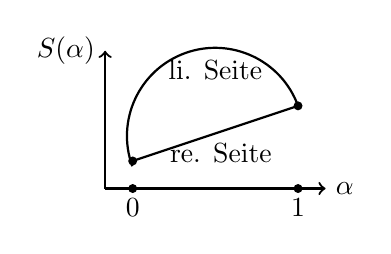
\begin{tikzpicture}[scale=0.7]
            \draw[->,thick](0,0) -- (4,0) node[anchor=west]{$\alpha$};
            \draw[->,thick](0,0) -- (0,2.5) node[anchor=east]{$S(\alpha)$};
            \filldraw[black] (0.5,0.5) circle (2pt);
            \filldraw[black] (3.5, 1.5) circle (2pt);
            \filldraw[black] (0.5,0) circle (2pt) node[anchor=north]{0};
            \filldraw[black] (3.5,0) circle (2pt) node[anchor=north]{1};
            \draw[-,thick](0.5,0.5) -- (3.5,1.5);
            \draw[-, thick](3.5,1.5) arc (20:200:1.6);
            \draw[] (2,2.5) node[anchor=north]{li. Seite};
            \draw[] (2.1,1) node[anchor=north]{re. Seite};
        \end{tikzpicture}
        \end{center}
        \item[] Bedeutung: Mischung von Verteilungen erhöht Entropie (Mischungsentropie) 
    \end{itemize}
\end{enumerate}
\end{prop}



\subsubsection{statistische Entropie eines quantenmechanischen Makrozustands}
\textbf{Falsch:} $\hat{\varrho} = \sum_n w_n \ket{\Psi_n}\bra{\Psi_n} \ \Rightarrow \ S(\hat{\varrho}) = -k\cdot\sum_n w_n \ln{w_n} $\\
\textbf{Problem:} Viele Kombinationen $\{w_n\, , \,\ket{\Psi_n}\}$ ergeben gleichen Dichteoperator $\hat{\rho} \ \Rightarrow \ S(\hat{\varrho})$ darf nur von $\hat{\varrho}$ abhängen und nicht von den verschiedenen $\{w_n\, ,\, \ket{\Psi_n}$.

\textbf{Richtig:} 
\begin{definition}{statistische Entropie eines qm Zustands}
    \begin{equation}
    S(\hat{\varrho}) = -k \cdot \trace (\hat{\varrho} \ln{\hat{\varrho}}) = -k \ \langle\ln{\hat{\varrho}}\rangle
    \end{equation}
\end{definition}

Wähle Eigenzustände von $\hat{\varrho}$ aus Basis für die Spur:
\begin{equation}
    \hat{\varrho} \ket{\varphi_n} = p_n \ket{\varphi_n}
\end{equation}


\begin{equation}
    \Rightarrow \ \ S(\hat{\rho}) = -k \cdot \sum_n \bra{\varphi_n} \hat{\varrho} \ln\hat{\varrho} \ket{\varphi_n} = -k \cdot \sum_n p_n \ln{p_n}
\end{equation}

\textbf{wichtig:} $p_n$ sind Eigenwerte zu $\hat{\varrho}$! 

\subsubsection*{Reiner Zustand:}
$\hat{\varrho}^2 = \hat{\varrho}$ anwenden auf $\ket{\varphi_n}$ (Eigenzustand von $\varrho$)

\begin{align}
    \Rightarrow \ \forall n: \ &&\hat{\varrho}^2 \ket{\varphi_n} = \hat{\varrho} \ket{\varphi_n}  \\
    \Rightarrow \ \forall n: \ &&p_n^2 \ket{\varphi_n} = p_n \ket{\varphi_n} \\
    \Rightarrow \ \forall n: \  &&p_n^2= p_n \\
    \Rightarrow \  \forall n: \  &&p_n = 0 \text{ oder } p_n = 1 \\
\end{align}
 \begin{equation}
   \Rightarrow \  \  S(\hat{\varrho}) = 0 , \text{ da volle Information}  
 \end{equation}
 
\subsubsection*{Gemischter Zustand:}
$\hat{\varrho}^2 \neq \varrho$
\begin{align}
    &\exists \ n:  \ &&p_n^2 = p_n\\
    \Rightarrow \ &\exists \ n:  \ &&0 < p_n < 1 \\
    \Rightarrow \ &S(\hat{\varrho}) > 0 \ &&\text{, d.h. Information fehlt!}
\end{align}
Maximale Entropie: \ \ Gleichverteilung $p_n = \frac{1}{M} \ \Rightarrow \ S = k \ln M$

\subsubsection{Statistische Entropie eines klassischen Makrozustands}

WS-Dichte $\varrho ( \Vec{q}, \Vec{p})$ im Phasenraum ist Funktion der kontinuierlichen Variablen $\Vec{q}, \Vec{p}$

$\Rightarrow$ keine diskreten WS $p_i \ \Rightarrow$ Problem

Betrachte Phasenraumzellen $\Gamma_i$ mit Volumina $\tau$ \\
$\Rightarrow$ diskrete WS $p_i$

\begin{equation}
    p_i = \int_{\Gamma_i} d\Vec{q} \, d\Vec{p}_i \ \varrho (\Vec{q}, \Vec{p}) \overset{(*)\text{\tiny{ $\varrho$ glatt}}}{\approx} \tau \varrho (\Vec{q}, \Vec{p}) \ \text{ für Punkt } (\Vec{q}, \Vec{p}) \in \Gamma_i
\end{equation}
(*) Wenn $\varrho$ glatt, dann ist es auf kleiner Umgebung von $(\Vec{q}_i,\Vec{p}_i)$ konstant und man $\varrho $ vor das Integral ziehen. (Hier wird angenommen, dass diese Bedingung immer erfüllt ist. Das ist sinnvoll, da $ h \sim 10^{-34}$ sehr kleine Größenordnung. \\
Bedingung ist beispielsweise bei multifraktalen WS-Verteilungen nicht erfüllt.)\\

$\Rightarrow$ statistische Entropie einer WS-Dichte im Phasenraum: \\
\begin{equation}
    S\bigl(\varrho(\Vec{q}, \Vec{p})\bigr) \approx -k \cdot\sum_i \tau \ \varrho(\Vec{q}_i,\Vec{p}_i)\ln \bigl(\tau \varrho (\Vec{q}_i, \Vec{p}_i)\bigr)
\end{equation}

\begin{definition}{Entropie}
    \begin{equation}
        S \bigl(\varrho ( \Vec{q},\Vec{p}) \bigr) = - k \ \int_\Gamma d\Vec{q} \, d\Vec{p} \ \varrho(\Vec{q},\Vec{p}) \ \ln{\bigl(\tau \ \varrho(\Vec{q},\Vec{p}\bigr)}
    \end{equation}
    
\end{definition}

\textbf{Probleme:}
\begin{itemize}
    \item[-] Abhängig von $ \tau$, divergiert für $\tau \rightarrow 0$
    \item[$\Rightarrow$] Lösung: Heisenbergsche Unschärferelation $\Delta q \Delta p \geq \frac{\hbar}{2}$
    \item[$\Rightarrow$] Elementarzelle $\tau \sim \hbar^f$ \ (f... Anzahl der Freiheitsgrade)
\end{itemize}

später: Planck-Zelle $\tau = h^f$

\begin{beispiel}{Beispiel: Gleichverteilung}
    Sei $\varrho=$ const. im Volumen $\Gamma$ des Phasenraums $\Rightarrow \ \varrho = \frac{1}{\Gamma}$ \\
    Zahl der Planck-Zellen: \ $M = \frac{\Gamma}{\tau} \ \Rightarrow \ \tau \varrho = \frac{\Gamma}{M} \frac{1}{\Gamma} = \frac{1}{M}$
    \begin{equation*}
        \Rightarrow \ S(\varrho = \text{ const. }) = -k \ \ln{\frac{1}{M}} \underbrace{\int_\Gamma d\Vec{q} \, d\Vec{p} \ \varrho(\Vec{q},\Vec{p})}_{=1} = k \ln M
    \end{equation*}

    \textbf{Bemerkung:} 
    \begin{itemize}
        \item[-] Entropie mit diskreten WS natürlich definiert
        \item[-] in klassischer Mechanik muss $\underbrace{\text{Planck-Zelle}}_{\text{sinnvoll, wegen Heisenberg Unschärfe}}$ eingeführt werden. (In qm ist das Konzept von Trajektorien bzw. Punkten im Phasenraum aufgrund der Unschärferelation nicht vorgesehen.)
    \end{itemize}
\end{beispiel}

\subsection{Gleichgewichtsensemble und Prinzip der maximalen Ensemble} \marginpar{VL 6}
Zustand eines Systems im themodynamischen Gleichgewicht $\Bigl( \frac{\partial \hat{\varrho}}{\partial t} = 0 \Bigr)$ charakterisiert durch:
\begin{itemize}
    \item Erhaltungsgrößen: Energie, Gesamtimpuls, Gesamtdrehimpuls, Teilchenzahl
    \item äußere Parameter: Volumen, Druck, Temperatur
\end{itemize}

System ist durch Wände begrenzt:
\begin{itemize}
    \item[$\Rightarrow$] Gesamtdrehimpuls und Gesamtimpuls nicht erhalten
    \item[$\Rightarrow$] Energie und Teilchenzahl möglich Erhaltungsgrößen
\end{itemize}

Die 3 wichtigsten Gleichgewichts-Ensemble sind: (\emph{$\rightarrow$ experimentell schwierig: Energie erhalten und Teilchenzahl nicht $\rightarrow$ 3 Möglichkeiten})

\begin{enumerate}
    \item \underline{Mikrokanonisches Ensemble:} \\
    isoliertes System:
    \begin{itemize}
        \item feste Energie $E$
        \item feste Teilchenzahl $N$
    \end{itemize}
    \item \underline{kanonisches Ensemble:} \\
    Austausch von Energie mit Umgebung $\Rightarrow$ Energie fluktuiert
    \begin{itemize}
        \item mittlere Energie $\langle E \rangle$ stellt sich ein; abhängig von Umgebung (insbesondere Temperatur)
        \item Teilchenzahl $N$ fest
    \end{itemize}
    \item \underline{Großkanonisches Ensemble}
    Austausch von Energie und Teilchen mit Umgebung
    \begin{itemize}
        \item[$\Rightarrow$] Energie und Teilchenzahl funktioniert
        \item mittlere Energie $\langle E \rangle$
        \item mittlere Teilchenzahl $\langle N \rangle$ stellt sich ein. Beides ist abhängig von der Umgebung
    \end{itemize}
\end{enumerate}

Welcher Dichteoperator $\hat{\varrho}$ beschreibt den Makrozustand zum jeweiligen Gleichgewichts-Ensemble?
\begin{equation*}
    \Longleftrightarrow
\end{equation*}
Was sind die Wahrscheinlichkeiten $p_n$ der Energie-Eigenzustände $E_n$?

\begin{prop}{Prinzip der maximalen Entropie (Jaynes, 1957)}
    Makrozustand im thermodynamischen Gleichgewicht wird mit dem Dichteoperator $\hat{\varrho}$ beschrieben, der die Entopie unter Einhaltung der Nebenbedingungen (z.B. mittlere Energie) \textbf{maximiert}.
\end{prop}

\underline{Bemerkung:}
\begin{itemize}
    \item Es wird nur die bekannte Information benutzt
    \item Jeder andere Dichteoperator $\hat{\varrho}$ mit kleinerer Entropie beinhaltet mehr Information über das System
\end{itemize}

\subsection{Mikrokanonisches Ensemble}\label{seq.Mikrokanonisches_ensemble}
Isoliertes System mit fester Energie $E$ und fester Teilchenzahl $N$.
\begin{center}
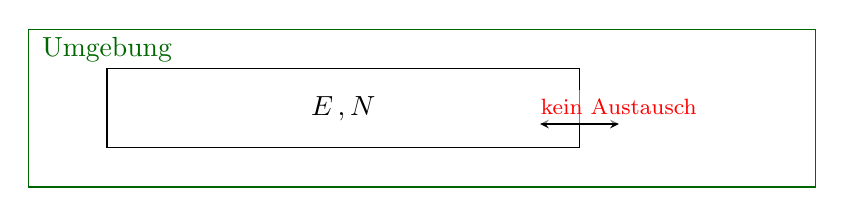
\begin{tikzpicture}
    \draw[green!40!black] (0,0)--(10,0)--(10,2)--(0,2)--(0,0);
    \draw (1,0.5)--(7,0.5)--(7,1.5)--(1,1.5)--(1,0.5);
    \draw[stealth-stealth] (6.5,0.8)--(7.5,0.8) node[above, red, fill=white,opacity=.5,text opacity=1] {\footnotesize{kein Austausch}};
    \draw (4,1) node {$E\, ,N$};
    \draw (1,1.75) node[green!40!black] {Umgebung};
\end{tikzpicture}
\end{center}

Teilchenzahl $N$ als diskrete Variable wird exakt angenommen; Energie $E$ ist kontinuierliche Variable
\begin{itemize}
    \item zu vorgegebener Energie $E$ gibt es i.A. keinen Mikrozustand mit $E_n = E$
    \item physikalische Messung ist mit Unsicherheit $\Delta E$ verbunden
    \item[$\Rightarrow$] Man betrachtet ein Energieintervall $[E-\Delta E,E]$ mit:
    \begin{enumerate}
        \item $\Delta E \ll E$
        \item $\Delta E$ groß genug, damit es viele Mikrozustände im Intervall gibt
        \item Vorhersagen sollten nicht von $\Delta E$ abhängen
    \end{enumerate}
\end{itemize}

Wie groß ist WS $p_n$ für Mikrozustand (=Energie-Eigenzustand) $\ket{\phi_n}$ mit $E_n \in [E-\Delta E,E]$?
\begin{itemize}
    \item[] Prinzip der maximalen Entropie mit Nebenbedingung: $\sum_n \ p_n = 1$
    \begin{equation}
        \stackrel{\equa{Geichverteilung}}{\Longrightarrow} \text{Gleichverteilung mit } p_n = const.
    \end{equation}
    \item[] (äquivalentes Postulat: alle Eigenzustände $\ket{\phi_n}$ eines isolierten Systems mit $E_n \in [E-\Delta E,E]$ haben gleiche Wahrscheinlichkeit. Es gibt keinen Grund, einen der Eigenzustände gegenüber anderen hervorzuheben.)
\end{itemize}

\paragraph{WS im mikrokanonischen Ensemble}
\begin{equation}
    p_n = \begin{cases}
        \frac{1}{M_{\Delta}(E)} \qquad \text{; falls } E_n \in [E-\Delta E,E] \\
        0 \qquad \text{; sonst}
    \end{cases}
\end{equation}
$M_{\Delta}(E)$ ist die Zahl der Zustände in $[E-\Delta E,E]$

\paragraph{Dichteoperator im mikrokanonischen Ensemble}
\begin{equation}
    \hat{\varrho} \ = \ \sum_n \ p_n \ \ket{\psi_n} \bra{\psi_n} \ = \ \frac{1}{M_{\Delta}(E)} \ \sum_{\substack{n \\ E_n \in [E-\Delta E,E]}} \ \ket{\psi_n} \bra{\psi_n}
\end{equation}
\begin{equation}
    \text{Test: } \trace(\hat{\varrho}) = \frac{1}{M_{\Delta}(E)} \ \sum_{\substack{n \\ E_n \in [E-\Delta E,E]}} \ \underbrace{\trace(\ket{\psi_n} \bra{\psi_n})}_{\braket{\psi_n}=1} \ = \ 1 \qquad \checkmark
\end{equation}

\paragraph{Mittelwerte im mikrokanonischen Ensemble}
\begin{equation}
    \langle \hat{A} \rangle = \trace(\hat{\varrho} \hat{A}) = \frac{1}{M_{\Delta}(E)} \ \sum_{\substack{n \\ E_n \in [E-\Delta E,E]}} \ \underbrace{\trace(\ket{\psi_n} \bra{\psi_n} \hat{A})}_{= \trace(\bra{\psi_n} \hat{A} \ket{\psi_n})}
\end{equation}
anschaulich: Mittelwert der Erwartungswerte

\paragraph{Dichteoperator im Limes $\Delta E \to 0$}
\begin{equation}
    \hat{\varrho} = \frac{\delta(E-H)}{\trace(\delta(E-H))}
\end{equation}

\paragraph{WS-Dichte im klassischen Phasenraum}
\begin{equation}
    \varrho(\Vec{q},\Vec{p}) = \frac{\delta(E-H(\Vec{q},\Vec{p}))}{\int d\Vec{q} \int d\Vec{p} \ \delta(E-H(\Vec{q},\Vec{p}))}
\end{equation}
$\delta$-Funktion auf Energieschale
\begin{center}
    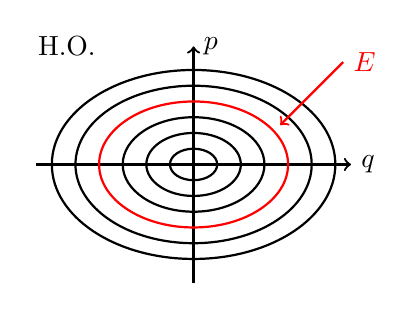
\begin{tikzpicture}
        \draw[->, thick] (-2,0) -- (2,0) node[anchor=west]{$q$};
        \draw[->, thick] (0,-1.5) -- (0,1.5) node[anchor=west]{$p$};
        \draw[] (-2.1, 1.5) node[anchor=west]{H.O.};
        \draw[thick] (0,0) ellipse (0.3 and 0.2);
        \draw[thick] (0,0) ellipse (0.6 and 0.4);
        \draw[thick] (0,0) ellipse (0.9 and 0.6);
        \draw[red, thick] (0,0) ellipse (1.2 and 0.8);
        \draw[thick] (0,0) ellipse (1.5 and 1.0);
        \draw[thick] (0,0) ellipse (1.8 and 1.2);
        \draw[<-, thick, red] (1.1,0.5) -- (1.9,1.3) node[anchor=west]{$E$};
    \end{tikzpicture}
\end{center}

\subsubsection{Zustandssumme, Zustandsdichte}
\emph{(ab jetzt: Mikrozustand = Energie-Eigenzustand = Zustand)}

\begin{center}

    \begin{tikzpicture}
    \draw[thick,->] (0,0) -- (5,0) node[anchor=north west] {$E$};
\draw[thick,->] (0,0) -- (0,3.5) node[anchor=south east] {$M_{\Delta}(E)$};
    \foreach \x in {0,1,2,3,4}
   \draw (\x cm,1pt) -- (\x cm,-1pt) node[anchor=north] {};
    \foreach \y in {0,1,2,3}
    \draw (1pt,\y cm) -- (-1pt,\y cm) node[anchor=east] {$\y$};
    \draw[red] (0,1)--(1.2,1)--(1.2,2)--(2.8,2)--(2.8,3)--(4.4,3);
    \draw (1.2,1pt)-- (1.2,-1pt)node[anchor=north] {$E_1$};
    \draw (2.8,1pt)-- (2.8,-1pt)node[anchor=north] {$E_2$};
    \draw (4.4,1pt)-- (4.4,-1pt)node[anchor=north] {$E_3$};
    \end{tikzpicture}

    \begin{tikzpicture}
    \draw[thick,->] (0,0) -- (5,0) node[anchor=north west] {$E$};
\draw[thick,->] (0,0) -- (0,3.5) node[anchor=south east] {$d(E)$};
    \foreach \x in {0,1,2,3,4}
   \draw (\x cm,1pt) -- (\x cm,-1pt) node[anchor=north] {};
    \foreach \y in {0,1,2,3}
    \draw (1pt,\y cm) -- (-1pt,\y cm) node[anchor=east] {$\y$};
    \draw (1.2,1pt)-- (1.2,-1pt)node[anchor=north] {$E_1$};
    \draw (2.8,1pt)-- (2.8,-1pt)node[anchor=north] {$E_2$};
    \draw (4.4,1pt)-- (4.4,-1pt)node[anchor=north] {$E_3$};
    \draw[red,->] (1.2,0)-- (1.2,3.5)node[anchor=north] {};
    \draw[red,->] (2.8,0)-- (2.8,3.5)node[anchor=north] {};
    \draw[red,->] (4.4,0)-- (4.4,3.5)node[anchor=north] {};
    \draw[-,thick,red] (0,0) -- (4.99,0);
    \end{tikzpicture}
\end{center}

\begin{definition}{Mikrokanonische Zustandssumme}
    \begin{align}
        Z &\coloneqq M(E) = \sum_n \ \Theta(E-E_n) \qquad \text{Anzahl der Zustände mit } E_n < E \\
        z &\coloneqq M_{\Delta}(E) = \sum_n \ \Theta(E - E_n) \Theta(E_n-(E-\Delta E)) \qquad \text{Anzahl mit } E_n \in [E- \Delta E, E]
    \end{align}
\end{definition}

\underline{Bemerkung:}
\begin{itemize}
    \item beide Definitionen unterscheiden sich bei großer Teilchenzahl nicht
    \begin{itemize}
        \item[Bsp.:] Volumen der Kugel vs Volumen einer Kugelschale an der Oberfläche
        \item[] in 3D vs in $6\cdot 10^{23}$D
    \end{itemize}
    \item kanonische und großkanonische Zustandssumme haben andere Definitionen
\end{itemize}

\begin{definition}{Zustandsdichte}
    \begin{equation}
        d(E):= \frac{d \ M(E)}{d \ E} = \sum_n \delta(E-E_n)
    \end{equation}
\end{definition}

\begin{beispiel}{Rechenbeispiel}
    \begin{equation}
        \int_{-\infty}^E dE^\prime \ d(E^\prime) = \int_{-\infty}^E dE^\prime \ \sum_n \delta(E_n -E^\prime)= \sum_n\ \int_{-\infty}^E dE^\prime \ \delta(E_n -E^\prime) = \sum_{\overset{n}{E_n<E}} 1 = M(E)
    \end{equation}
\end{beispiel}

\marginpar{VL 7}
\subsubsection{Ideales Gas}\label{seq.ideales Gas}
\begin{itemize}
    \item $N$ Teilchen, Masse $m$, Volumen $V$
    \item keine WW, punktförmig, keine innere Struktur (einatomig)
    \item Hamilton-Fkt., Hamilton-Operator
    \begin{equation}
        H = \sum_{j=1}^N \frac{\Vec{p_j}^2}{2m} \qquad \Vec{q} \in V
    \end{equation}
    \item[Ziele]:
    \begin{itemize}
        \item Bestimme Zahl der Zustände qm und klassisch
        \item Vergleich $\Rightarrow$ Größe der Planck-Zelle
    \end{itemize}
\end{itemize}

\paragraph{Quantenmechanisches ideales Gas}
Energie-Eigenzustände:
\begin{itemize}
    \item 1D, N = 1: Quantenzahl n = 1,2,...
    \begin{align}
        \varphi_n(x) &= A_1 \cdot sin\left(\frac{\pi}{L} n x \right) \\
        E_n &= \frac{\hbar^2}{2m} \left(\frac{\pi}{L} n \right)^2 = \frac{h^2}{8mL^2} n^2
    \end{align}
    
    \begin{center}
    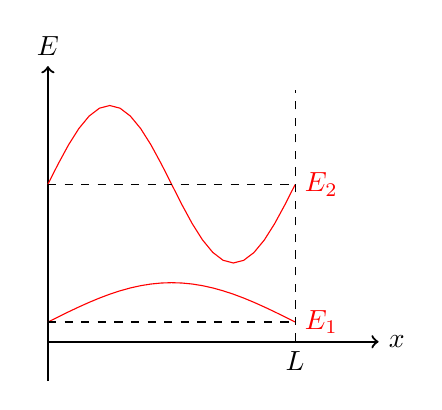
\begin{tikzpicture}[domain=0:3.14]
  \draw[->, thick] (-0.01,0) -- (4.2,0) node[right] {$x$};
  \draw[->, thick] (0,-0.5) -- (0,3.5) node[above] {$E$};
  \draw[color=red]   plot (\x,{0.5*(sin(\x r)+0.5)})    node[right] {$E_1$};
  \draw[color=red] plot (\x,{sin(\x*2 r)+2}) node[right] {$E_2$};
  \draw[dashed] (3.14,0) --(3.14,3.2);
  \draw[dashed] (0,0.25) --(3.14,0.25);
  \draw[dashed] (0,2) --(3.14,2);
  \node[below] at (3.14,0) {$L$};
\end{tikzpicture}
\end{center}

    \item 3D, N=1: Quantenzahlen $n_x,n_y,n_z$ ($L_x=L_y=L_z=L$)
    \begin{align}
        \varphi_{n_x,n_y,n_z}(\Vec{r}) &= A_3 \cdot sin\left(\frac{\pi}{L} n_x x \right)  sin\left(\frac{\pi}{L} n_y y \right)  sin\left(\frac{\pi}{L} n_z z \right) \\
        E_{n_x,n_y,n_z} &= \frac{h^2}{8mL^2} \underbrace{(n_x^2 + n_y^2 +n_z^2)}_{\text{3D-Gitter mit Abstand 1}}
    \end{align}
    
    \begin{figure*}
    \centering
    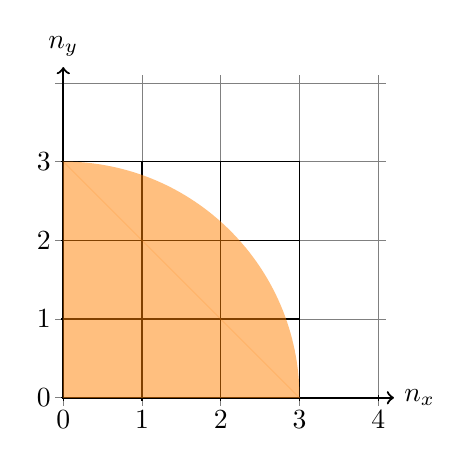
\begin{tikzpicture}
     \draw[very thin,color=gray] (-0.1,-0.1) grid (4.1,4.1);
     \foreach \y in {0,1,2,3}
    \draw (1pt,\y cm) -- (-1pt,\y cm) node[anchor=east] {$\y$};
    \foreach \x in {0,1,2,3,4}
   \draw (\x cm,1pt) -- (\x cm,-1pt) node[anchor=north] {$\x$};
    \draw[->, thick] (-0.01,0) -- (4.2,0) node[right] {$n_x$};
  \draw[->, thick] (0,-0.01) -- (0,4.2) node[above] {$n_y$};
   \draw (0.5,0.5) node[minimum height=1cm,minimum width=1cm,draw] {};
   \draw (0.5,1.5) node[minimum height=1cm,minimum width=1cm,draw] {};
   \draw (0.5,2.5) node[minimum height=1cm,minimum width=1cm,draw, fill=white] {};
   \draw (2.5,0.5) node[minimum height=1cm,minimum width=1cm,draw, fill=white] {};
   \draw (1.5,0.5) node[minimum height=1cm,minimum width=1cm,draw, fill=white] {};
   \draw (1.5,1.5) node[minimum height=1cm,minimum width=1cm,draw, fill=white] {};
   \draw (1.5,2.5) node[minimum height=1cm,minimum width=1cm,draw, fill=white] {};
   \draw (2.5,1.5) node[minimum height=1cm,minimum width=1cm,draw, fill=white] {};
   \draw (2.5,2.5) node[minimum height=1cm,minimum width=1cm,draw, fill=white] {};
   \draw[thick, red, fill=orange,opacity=.5, draw=none] (3,0) arc (0:90:3);
   \filldraw[fill=orange, opacity =.5, draw=orange, draw opacity = .1] (0,0) -- (0,3) -- (3,0);
    \end{tikzpicture}
    \caption{Abzählung der Zustände in 2D}
\end{figure*}

    \item 3D, N: Quantenzahlen $n_{1x},n_{1y},n_{1z},n_{2x},\dots, n_{Nz}$
    \begin{align}
        E_{n_{1x},\dots,n_{Nz}} = \frac{h^2}{8mL^2} &\underbrace{(n_{1x}^2 + \dots + n_{Nz})}_{(\text{Abstand vom Ursprung})^2} \\ 
        &_\text{in 3N-dim. Gitter mit Gitterabstand 1}
    \end{align}
\end{itemize}

Zahl der Zustände mit Energie kleiner $E$:
\begin{equation}
    M(E) = \frac{V_{3N}\left(\sqrt{\frac{8mL^2 E}{h^2}}\right)}{\underbrace{1^{3N}}_{\text{Einheitszelle}}} \cdot \underbrace{\left( \frac{1}{2}\right)^{3N}}_{\text{\glqq Viertelkreis \grqq}}
\end{equation}

Volumen der f-dim. Kugel mit Radius $R$:
\begin{equation}
    V_f(R) = c_f \cdot R^f \qquad c_f = \frac{\pi^{f/2}}{\frac{f}{2}\Gamma(\frac{f}{2})}
\end{equation}
\begin{center}
\fcolorbox{red}{white}{
\begin{equation}
    \hspace{2cm} M(E) \quad = \quad c_{3N} \left( \frac{8 m L^2 E}{h^2}\right)^{\frac{3N}{2}} \frac{1}{2^{3N}} \quad  = \quad c_{3N} \frac{1}{h^{3N}} (2m)^{\frac{3N}{2}} V^N E^{\frac{3N}{2}} \hspace{2cm}
\end{equation}
}
\end{center}
\textbf{Bemerkung:}
\begin{enumerate}
    \item Ununterscheidbarkeit nicht berücksichtigt $\Rightarrow$ Formel bei Diskussion Quantengase korrigiert
    \begin{itemize}
        \item unterschiedliche Ausdrücke für Fermionen und Bosonen
        \item Grenzfall: WS Besetzung eines Zustands $\ll 1$ (Maxwell-Boltzmann-Näherung)
        \item[$\Rightarrow$] Korrekturfaktor $\frac{1}{N!}$ 
    \end{itemize}
    \item Extrem starke Zunahme mit $E$
    \item Vergleiche beide Definitionen der mikrokanonischen Zustandssumme $Z = M(E)$ und $y = M_\Delta (E) = M(E) -M(E_\Delta)$:
    \begin{align}
        \frac{z}{Z} = \frac{M_\Delta(E)}{M(E)} = 1 - \frac{M(E-\Delta)}{M(E)} = 1 -\frac{(E-\Delta)^{3N/2}}{E^{3N/2}} = 1- \Bigl( 1- \frac{\Delta}{E}\Bigr)^{3N/2}  \\
        = 1- e^{\ln(^-\frac{\Delta}{E})^{3N/2}} = \underbrace{1- e^{\frac{3N}{2} \ \ln{(1-\frac{\Delta}{E})}}}_{\text{Taylorentwicklung: } \ln (1-\frac{\Delta}{E}) \approx -\frac{\Delta}{E}} \overset{\Delta \ll E}{=} 1- e^{\frac{3N}{2} \frac{\Delta}{E}}
    \end{align}
\end{enumerate}

Fallunterscheidung:
\begin{itemize}
    \item[-] \underline{$\frac{N \Delta}{E} \ll 1$:} $\Leftrightarrow \ \ \frac{\Delta}{E} \ll \frac{1}{N} \ \ \Leftrightarrow \ \ \Delta \ll \frac{E}{N}$ (mittlere Energie pro Teilchen): \\
    \begin{equation}
        \frac{M_\Delta(E)}{M(E)} \approx 1- \Bigl( 1- \frac{3N}{2} \frac{\Delta}{E} \Bigr)= \frac{3N}{2} \frac{\Delta}{E}
    \end{equation}
    \item[-] \underline{$1 \ll \frac{N \Delta}{E}:$} $\Leftrightarrow \ \ \frac{1}{N} \ll \frac{\Delta}{E} \ll 1 \ \ \Leftrightarrow \ \ \frac{E}{N} \ll \Delta \ll E$
    \begin{equation}
        \frac{M_\Delta(E)}{M(E)} \approx 1
    \end{equation}
    unabhängig von $\Delta$
    \item[-] \underline{$\frac{N\Delta}{E} \approx 1$:} keine Näherung möglich! 
    \item[$\rightarrow$] $N = 10^{23} \ \ \Rightarrow$ Bereich riesig: Messfehler ist in diesem Bereich
     \item[$\Rightarrow$] Physikalisch relevanter Bereich
      \item[$\rightarrow$] Zahl der Zustände $M_\Delta(E) \approx M(E)$ (mikrokanonische Zustandssumme $z \approx Z$)
       \item[$\rightarrow$]mikrokanonisches Ensemble berücksichtigt fast alle Zustände $E_n < E$
\end{itemize}

\paragraph{klassisches ideales Gas}
\begin{align}
    M(E) &= \frac{\text{\footnotesize{erlaubtes Phasenvolumen}}}{\text{\footnotesize{Volumen der Planck-Zelle}}} = \frac{\int_{H (\Vec{q},\Vec{p}) < E} d\Vec{q}\, d\Vec{p}}{\tau} \underbrace{\frac{1}{N!}}_{\text{Ununterscheidbarkeit- Gibbs-Paradoxon}} \\
    &= \frac{1}{N! \tau} \int d\Vec{q} \, d\Vec{p} \ \Theta\bigl(E-H(\Vec{q}, \Vec{p})\bigr) \\
    &= \frac{1}{N! \tau} \underbrace{\int_0^L dq_1 \dots \int_0^L dq_{3N}}_{L^{3N}= V^N} \underbrace{\int_{-\infty}^\infty dp_1 \dots \int_{-\infty}^\infty dp_{3N} \ \Theta\bigl( E- \sum_{i=1}^{3N} \frac{p_i^2}{2m}\bigr)}_{V_{3N}\bigl(\sqrt{2mE}\bigr) = c_{3N} \, (2mE)^{\frac{3N}{2}}}\\
    &=c_{3N} \, \frac{1}{N! \, \tau} \, (2m)^{\frac{3N}{2}} \, V^N \, E^\frac{3N}{2}
\end{align}
Vergleich klassische und quantenmechanische Rechnung für dieses Bsp.:
\begin{center}
    \fcolorbox{red}{white}{$\tau = h^{3N}$}
\end{center}
 ist Volumen der Planck-Zelle

 \subsection{kanonisches Ensemble}\label{sec.Kanonisches Ensemble} \marginpar{VL 8}
 konstante Teilchenzahl $N$; Energieaustausch mit Umgebung.
 $\Rightarrow$mittlere Energie $\langle E\rangle$ stellt sich ein.

 \begin{center}
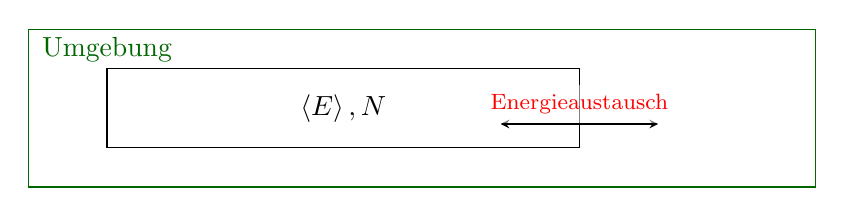
\begin{tikzpicture}
    \draw[green!40!black] (0,0)--(10,0)--(10,2)--(0,2)--(0,0);
    \draw (1,0.5)--(7,0.5)--(7,1.5)--(1,1.5)--(1,0.5);
    \draw[stealth-stealth] (6,0.8)--(8,0.8) node[above,midway, red, fill=white,opacity=.5,text opacity=1] {\footnotesize{Energieaustausch}};
    \draw (4,1) node {$\langle E\rangle \, ,N$};
    \draw (1,1.75) node[green!40!black] {Umgebung};
\end{tikzpicture}
\end{center}

\begin{itemize}
    \item[]Welche Dichteopeator $\varrho$ beschreibt den Mikrozustand?\tikzmark{start}
    \item[] Wie groß ist die WS $p_n$ für Eigenstustand $\ket{\varphi_n}$ Eigenenergie $E_n$ ?\tikzmark{end}
\end{itemize}

 
 \begin{tikzpicture}[remember picture,overlay]
    \draw[decorate,decoration={calligraphic brace}]
        ([yshift=10pt,xshift=10pt]{{pic cs:end}|-{pic cs:start}}) --
        node[xshift=5pt,anchor=west, text width=4cm] {identisch im \\ thermodynamischen Gleichgewicht}
        ([xshift=10pt]{pic cs:end})
;
\end{tikzpicture}

\subsubsection{Maximierung Entropie}

Entropie: 
\begin{equation}
    S=-k \trace\left(\varrho \ln \varrho\right)
\end{equation}
\begin{itemize}
    \item Variation von $\varrho$ unter Nebenbedingung
    \begin{equation}
        \trace(\varrho) =1
    \end{equation}
    \item Weitere Nebenbedingung
    \begin{equation}
        \trace(\varrho A_i) =\langle A_i \rangle
    \end{equation}
    \item[$\rightarrow$] kanonisches Ensemble ($i=1)$:  
    \begin{align}
        A_1 &=H & \langle A_1\rangle&=\langle H\rangle=\langle E\rangle
    \end{align}
    \item[$\rightarrow$] großkanonisches Ensemble ($i=2$):
    \begin{align}
        A_1 &=H & \langle A_1\rangle&=\langle H\rangle=\langle E\rangle\\
        A_2 &= \hat{N} \text{ Teilchenzahl}& \langle A_2\rangle&= \langle N\rangle \text{ mittlere Teilchenzahl}
    \end{align}
\end{itemize}

Nutze Methode der Lagrange-Multiplikatoren \ref{lagrange}\\
$\Rightarrow$ Maximiere:
\begin{equation}
    \Tilde{S} \left(\varrho, \lambda, ,\ \{\lambda_i\}\right) = -k \color{black!30!white}\Bigl( \color{black} \trace \left( \varrho \ln\varrho \right) +\lambda\left( \trace \varrho -1\right) + \sum_i \lambda_i \left( \trace(\varrho A_i) -\langle A_i\rangle \right)  \color{black!30!white}\Bigr) \color{black}
\end{equation}
(Die grauen klammern werden einfach eingefügt. Sie verändern nur die Lagrange-Multiplikatoren. Die Rechnung wird aber erleichtert)

\begin{enumerate}
    \item[0. Schritt] Ableitung nach $\lambda, \, \{\lambda_i\}$ ergibt Nebenbedingungen
    \item[1. Schritt] Suche stationären Punkt $\delta\Tilde{S} =0$ unter Nebenbedingung $\delta\varrho$:
    \begin{equation}
        \delta\Tilde{S} = -k \trace \Bigl( \delta \varrho  \underbrace{(\ln \varrho +1 + \lambda+\sum_i \lambda_i A_i)}_{\stackrel{!}{=}0} \Bigr)
    \end{equation}
    $\Rightarrow$ stationäre Lösung:
    \begin{equation}
        \varrho= e^{-1-\lambda -\sum_i \lambda_i A_i} =: \frac{1}{Z} e^{-\sum_i \lambda_i A_i}
    \end{equation}
    \item[2. Schritt] Entropie der stationären Lösung:
    \begin{align}
        S(\varrho)&= -k \trace(\varrho \ln \varrho) =-k \trace\left( \varrho( -\ln(Z) - \sum_i \lambda_i A_i )\right) \\
        &=k \ln(Z) \underbrace{\trace \varrho}_{=1} +k \sum_i \lambda_i \underbrace{\trace(\varrho A_i)}_{= \langle A_i\rangle}
    \end{align}
    \begin{equation}
      \fcolorbox{red}{white}{$S(\varrho) =k \ln (Z) + k \sum_i \lambda_i \ \langle A_I\rangle$}
    \end{equation} \color{black!50!white}
    \item[3. Schritt] zeige, dass $S$ maximal ist. -Wird hier nicht gezeigt. Man nutze $S(\Tilde{\varrho } ) \leq -k \trace(\Tilde{\varrho} \ln \varrho)$. Der Beweis verbleibt als Übung für die Lesenden.
\end{enumerate}
\color{black}

\textbf{Zusammenfassung}

\begin{definition}{Boltzmann-Gibbs-Verteilung}
    \begin{equation}
        \hat{\varrho} = \frac{1}{Z} \ e^{-\sum_i \lambda_i A_i }
    \end{equation}
\end{definition}

\begin{definition}{Zustandssumme}
    $\trace\varrho=1 \ \Rightarrow$
    \begin{equation}
        Z\left( \{ \lambda_i\}\right) = \trace\left( e^{-\sum_i \lambda_i A_i}\right)
    \end{equation}
\end{definition}

 \begin{definition}{Entropie}
     \begin{equation}
         S(\varrho) =k \ln (Z) + k \sum_i \lambda_i \ \langle A_i\rangle
     \end{equation}
 \end{definition}

\subsubsection{kanonischer Dichteoperator, Kanonische Zustandssumme}

kanonisches Ensemble: \hspace{2cm} $A_1 = H \ \ \lambda\rightarrow\beta$ \hspace{2cm} (später: $\beta=\frac{1}{k_BT}$)


\begin{align}
    \hat{\varrho} &= \frac{1}{Z} \ e^{-\beta H} \\
    Z(\beta)&= \trace \left( e^{-\beta \hat{H}} \right) \hspace{2cm} \text{kanonische Zustandssumme} \\
    S(\hat{\varrho}) &= k \ln (Z) + k \beta \langle E \rangle 
\end{align}

In der Basis der Energie-Eigenzustände $\ket{\varphi_n}:$
\begin{equation}
    p_n = \bra{\varphi_n}\hat{\varrho} \ket{\varphi_n} = \frac{1}{Z} \bra{\varphi_n} \underbrace{e^{-\beta \hat{H}}\ket{\varphi_n}}_{e^{-\beta E_n \ket{\varphi_n}}} = \frac{1}{Z} e^{-\beta E_n}
\end{equation}

\begin{equation}
    \fcolorbox{red}{white}{\hspace{2cm} $p_n = \frac{1}{Z} e^{-\beta E_n} \hspace{1cm} \xRightarrow[\sum_n p_n =1]{} \hspace{1cm} Z(\beta) = \sum_n e^{-\beta E_n}$ \hspace{2cm}}
\end{equation}

Erwartungswert im Gleichgewicht:
\begin{equation}
    \langle E\rangle = \trace (\varrho H ) = \sum_n \bra{\varphi_n} \underbrace{\varrho}_{\varrho= \sum_i p_i \ket{\varphi_i}\bra{\varphi_i}}H\ket{\varphi_n} =\sum_n p_n E_n
\end{equation}

\paragraph{Bemerkung}
\begin{itemize}
    \item Zustände mit gleicher Energie $E_n$ haben gleiche WS ($\widehat{=}$ mikrokaninisch.)
    \item alle Zustände (mit bel. Energie) haben WS > 0.
    \item $\sum_n$ ist Summe über Zustände (und nicht Energie $E_n$; Entartung!)
\end{itemize}

\paragraph{Allgemeine Bemerkung zu Boltzmann-Gibbs-Verteilung:}
\begin{enumerate}
    \item Erwarungswerte $\langle A_i\rangle$ aus Zustandssumme $Z\left( \{\lambda_i \}\right)$
    \begin{align}
        \langle A_i \rangle &= \trace (\varrho A_i ) = \trace \left( \frac{1}{Z} \, e^{-\sum_j \lambda_j A_j } A_i \right) = -\frac{1}{Z} \frac{\partial}{\partial \lambda_i} \underbrace{\trace\left( e^{-\sum_j \lambda_j A_j}\right)}_{Z} \\
        &= - \frac{\partial}{\partial \lambda_i} \ln \left( Z(\{\lambda_i\}\right)
    \end{align}
    \item Die Lagrange-Multiplikatoren $\lambda_i$ haben makroskopisch physikalische Interpretation $\rightarrow$ Umgebung
    \item Abhängigkeit der Entropie von Erwartungswerten
    \begin{align}
        \frac{\partial S \left( \langle A_i \rangle, \langle A_2 \rangle ,\dots \right)}{\partial \langle A_i \rangle} &= k \lambda_i & \frac{\partial S \left( \langle E \rangle\right)}{\partial \langle E \rangle}&= k \beta = \frac{1}{\beta}
    \end{align}
\end{enumerate}

\subsubsection{klassisches kanonisches Ensemble}
$f$ Freiheitsgrade $q_1, ... , q_f, \, p_1, ... , p_f, \, H(\Vec{q},\Vec{p})$

\begin{align}
    &\textbf{qm} &\longrightarrow \hspace{1cm} &\textbf{klass}\\
    \varrho &= \frac{1}{Z(\beta)} e^{-\beta H} &\longrightarrow \hspace{1cm}& \varrho(\Vec{q},\Vec{p}) = \frac{1}{Z(\beta)} e^{-\beta H(\Vec{q},\Vec{p})} \\
    \trace\varrho &=1 &\longrightarrow\hspace{1cm} &  \frac{1}{N!} \frac{1}{h^f} \int d\Vec{q} \, d\Vec{p} \ \varrho(\Vec{q}, \Vec{p}) =1 \\
    Z(\beta)&= \trace (e^{-\beta H}) &\longrightarrow\hspace{1cm} & Z(\beta) = \frac{1}{N!} \frac{1}{h^f} \int d\Vec{q} \, d\Vec{p} \ e^{- \beta H(\Vec{q},\Vec{p})} \\
    \langle A \rangle &= \trace(\varrho A) & \longrightarrow \hspace{1cm}& \langle A(\Vec{q}, \Vec{p}) \rangle = \frac{\int d\Vec{q} \, d\Vec{p} \ A(\Vec{q}, \Vec{p}) \ e^{- \beta H(\Vec{q},\Vec{p})} }{\int d\Vec{q} \, d\Vec{p} \ e^{- \beta H(\Vec{q},\Vec{p})}} \\
    %\frac{\frac{1}{N! \, h^f} \int d\Vec{q} \, d\Vec{p} \ e^{- \beta H(\Vec{q},\Vec{p})} }{\int d\Vec{q} \, d\Vec{p} \ e^{- \beta H(\Vec{q},\Vec{p})}} \\
    \text{speziell: } \langle H \rangle &= - \frac{d}{d \beta} \ln(Z(\beta)) & \longrightarrow \hspace{1cm}&\langle H \rangle = - \frac{d}{d \beta} \ln(Z(\beta)) 
\end{align}
Die Wahrscheinlichkeit für eine einzelne Koordinate $q_f \in [q_f, q_f + dq_f]$ ergibt sich zu:
\begin{align}
    w(q_f) \cdot dq_f &= \frac{1}{N! \, h^f} \int d\Vec{p} \ \int dq_1^{\prime} \dots \int dq_{f-1}^{\prime} \ dq_f^{\prime} \, \varrho(\Vec{q}^{\prime}, \Vec{p}) \\
    &= \frac{\int d\Vec{p} \ \int dq_1 \dots \int dq_{f-1} \ dq_f^{\prime} \, e^{- \beta \, H(\Vec{q}^{\prime}, \Vec{p})}}{\int d\Vec{p} \ \int dq_1^{\prime} \dots \int dq_{f-1}^{\prime} \ \int dq_f^{\prime} \, e^{- \beta \, H(\Vec{q}^{\prime}, \Vec{p})}}
\end{align}



\subsubsection{Gleichverteilungssatz} \marginpar{VL 9}
\emph{klassisch:} Sei in $H(\Vec{q},\Vec{p})$ ein quadratischer Term in $p_m$
\begin{align}
    H(\Vec{q},\Vec{p}) &= a \, p_m^2 + b \\
    \text{mit } a &= a(p_1, \dots, p_{m-1}, p_{m+1}, \dots, p_f,q_1,\dots, q_f) > 0 \\
    b &= b(p_1, \dots, p_{m-1}, p_{m+1}, \dots, p_f,q_1,\dots, q_f)
\end{align}
\emph{kanonisches Ensemble:}
\begin{align}
    \langle a \, p_m^2 \rangle &= \frac{\int d\Vec{q} \ \int d\Vec{p} \ a \, p_m^2 \, e^{-\beta(a p_m^2+b)}}{\int d\Vec{q} \ \int d\Vec{p} \ e^{-\beta(a p_m^2+b)}} \\
    &= \frac{\int d\Vec{q} \ \int dp_1 \dots \int dp_{m-1} \ \int dp_{m+1} \dots \int dp_f}{\int d\Vec{q} \ \int d\Vec{p} \ e^{-\beta(a p_m^2+b)}} \underbrace{\int_{\infty}^{\infty} dp_m \ p_m \ a \, p_m e^{-\beta(a p_m^2+b)}}
\end{align}
\begin{equation}
    \hspace{5cm} \stackrel{p.I.}{=} \underbrace{p_m \frac{e^{-\beta(a p_m^2 + b)}}{- 2 \beta}\Big|_{-\infty}^{\infty}}_{= 0} - \int_{-\infty}^{\infty} dp_m 1 \cdot \frac{e^{-\beta(a p_m^2 + b)}}{- 2 \beta}
\end{equation}
\begin{align}
   &= \frac{\int d\Vec{q} \ \int dp_1 \dots \int dp_{m-1} \ \int dp_{m+1} \dots \int dp_f}{\int d\Vec{q} \ \int d\Vec{p} \ e^{-\beta(a p_m^2+b)}} \frac{1}{2 \beta} \int_{-\infty}^{\infty} dp_m e^{-\beta(a p_m^2 + b)} \\
   &= \frac{1}{2 \beta} \color{black!50!white} = \frac{1}{2} k T \color{black} \rightarrow \text{Ergebnis unabhängig von a(\dots) und b(\dots)}
\end{align}

$\longrightarrow$ analog quaratischer Term in $q_m: \ H(\Vec{q},\Vec{p}) = a^{\prime} q_m^2 + b^{\prime}$
\begin{equation}
    \langle a^{\prime} q_m^2 \rangle = \frac{1}{2} k T
\end{equation}

\begin{definition}{Gleichverteilungssatz}
    Jeder unabhängige quadratische Term in $H(\Vec{q},\Vec{p})$ besitz den Erwartungswert $\frac{1}{2} k T$.
\end{definition}

\begin{beispiel}{Beispiel}
    \begin{itemize}
        \item 1D harmonischer Oszillator:
        \begin{align}
            H &= \frac{p^2}{2m} + \frac{1}{2} m \omega^2 q^2 \\
            &\Rightarrow \langle E \rangle = \langle E_{kin} \rangle + \langle E_{pot} \rangle = k T
        \end{align}
        \item 3D freies Teilchen:
        \begin{align}
            H &= \frac{p_x^2 + p_y^2 + p_z^2}{2 m} \\
            &\Rightarrow \langle E \rangle = \frac{3}{2} k T
        \end{align}
    \end{itemize}
\end{beispiel}



\subsubsection{Maxwellsche Geschwindigkeitsverteilung}
klassisches Gas im Potential $V(\Vec{p}).$\\

Betrachte 1 Teilchen im Wärmebad der anderen Teilchen (andere Teilchen $\widehat{=}$ Umgebung)\footnote{Frage aus Plenum: Ist diese Annahme, dass wir die anderen Teilchen als Umgebung betrachten sinnvoll? \\
Antwort:Ja. Das betrachtete Teilchen tauscht durch Stöße Energie mit den anderen Teilchen aus ($\widehat{=}$ Energieaustausch mit Umgebung.) Außerdem gilt globaler Energie- und Impulserhalt.\\
Das kanonische Ensemble kann angenommen werden, wenn sich die Umgebung nicht ändert. D.h. man muss warten, bis sich eine mittlere Energie $\langle E\rangle$ einstellt und sich die Umgebung damit zeitlich (statistisch) nicht mehr ändert.}

\begin{align}
    H(\Vec{q},\Vec{p}) &= \frac{\Vec{p}^2}{2m} + V(\Vec{q}) \\
    \varrho(\Vec{q},\Vec{p}) &= \frac{1}{Z} e^{- \beta H(\Vec{q},\Vec{p})} \propto e^{- \beta \left(\frac{\Vec{p}^2}{2m} + V(\Vec{q})\right)}
\end{align}

Impulsverteilung in einer Dimension:
\begin{equation}
    P(p_x) \propto e^{- \beta \frac{p_x^2}{2m}}
\end{equation}

\begin{center}
\begin{tikzpicture}
\begin{axis}[
    axis lines = left,
    xlabel = \(p_x\),
    ylabel = {\(P(p_x)\)},
     xticklabels={},
    yticklabels={}
]

\addplot [
    domain=-10:10, 
    samples=100, 
    color=red,
    line width=pt
]
{exp{-(0.3*x)^2}};
\end{axis}

\draw[<->] (2.35,2.4)--(4.5,2.4) node[above, midway] {$\sqrt{\frac{\beta}{m}}$};
\end{tikzpicture}   
\end{center}

Verteilung Betrag des Impulses: $p := \sqrt{\Vec{p}\cdot \Vec{p}}$
\begin{equation}
    P(p) \propto p^2 e^{-\beta \frac{p^2}{2m}}
\end{equation}

\begin{center}
    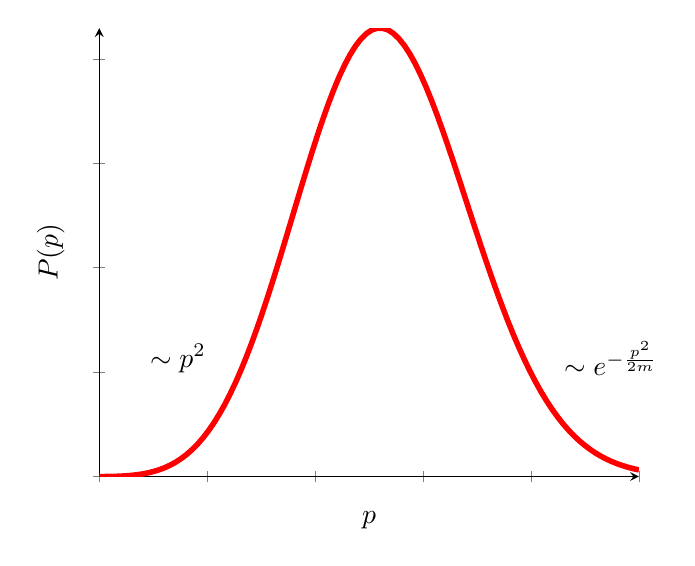
\begin{tikzpicture}
\begin{axis}[
    axis lines = left,
    xlabel = \(p\),
    ylabel = {\(P(p)\)},
     xticklabels={},
    yticklabels={}
]

\addplot [
    domain=0:10, 
    samples=100, 
    color=red,
    line width=2pt
]
{0.1*(x^2*exp{-(0.4*(x-4))^2})};

\end{axis}
\node[]at (1,1.5){$\sim p^2$};
\node[]at (6.5,1.5){$\sim e^{-\frac{p^2}{2m}}$};
\end{tikzpicture}
\end{center}



\begin{beispiel}{Bsp. in Vorlesung: Dynamische Animation mit 50 Teilchen im 2D-Billiard}
Zu Beginn haben alle Teilchen den gleichen Geschwindigkeitsbetrag.
    \begin{enumerate}
        \item Animation wird losgeschickt. Zuerst gibt es nach WW mit der Wand keine Veränderung des Impulsbetrags der Teilchen. Mit der Zeit wird Impulsverteilung breiter. Mit der Zeit stellt sich das Gleichgewicht ein und die Verteilung passt sich der theoretischen Kurve an.\\
        Da es um eine 2D-Verteilung handelt, skaliert die linke Seite der Kurve mit $p^1$. (Im 2D-Phasenraum können die Impulse als Oberfläche eines Kreisen ($\widehat{=}$ Kreisumfang $\approx p$) angenommen werden.)
  \begin{center}
    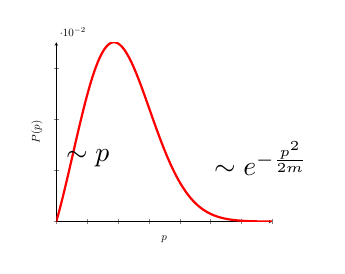
\begin{tikzpicture}[scale=0.4]
        
\begin{axis}[
    axis lines = left,
    xlabel = \(p\),
    ylabel = {\(P(p)\)},
     xticklabels={},
    yticklabels={},
]

\addplot [
    domain=0:35, 
    samples=100, 
    color=red,
    line width=2pt
]
{x*0.01*(exp{-(0.1*(x-4))^2})};

\end{axis}
\node[]at (1,2){$\sim p$};
\node[]at (6.5,2){$\sim e^{-\frac{p^2}{2m}}$};
\end{tikzpicture}
\end{center}
        

\item Nun gibt es Energieaustausch mit der Wand: Nach Stoß mit der Wand wird die Geschwindigkeit der Teilchen auf einen festen Betrag gesetzt, damit die Temperatur des Systems konstant bleibt. Nach einer gewissen Zeit stellt sich ein gleichgewicht Analog zu der eben gezeigten theoretischen Kurve ein. Allerdings gibt es einen weiteren Peak rechts des maximums: \\
Grund dafür ist, dass langsame Teilchen seltener zur Wand gelangen. Damit ist die durchschnittliche Geschwindigkeit, mit der Teilchen auf die Wand treffen, größer als die Durchschnittsgeschwindigkeit aller Teilchen.
\item Nun wird die Wand geheitzt. Nach einer gewissen Zeit stellt sich wieder ein Gleichgewicht ein.
        

\end{enumerate}
\end{beispiel}
\subsubsection{Energieverteilung im kanonischen Ensemble}
System habe eine Energie in $[E, E+ dE ]$. Wie groß ist WS $P(E) \ dE$?
\begin{align}
    P(E) \ dE &\propto \left[ M(E+dE) - M(E) \right] e^{- \beta E} \\
    \rightarrow \ P(E) &\propto \frac{dM(E)}{dE} e^{-\beta E} = \underbrace{d(E)}_{\text{Zustandsdichte}} \overbrace{e^{-\beta E}}^{\text{fällt für große E ab}}\\
    &\text{ideales Gas:  } d(E) \propto E^{\frac{3N}{2}-1} \\
    \Rightarrow &P(E) \text{ hat Minimum}
\end{align}

\begin{center}
\begin{tikzpicture}
\begin{axis}[
    axis lines = left,
    xlabel = \(E\),
    ylabel = {\(P(E)\)},
    xticklabels={},
    yticklabels={},every axis x label/.style={
    at={(ticklabel* cs:1.05)},
    anchor=west,},
every axis y label/.style={
    at={(ticklabel* cs:1.05)},
    anchor=south,}
]

\addplot [
    domain=0:7, 
    samples=100, 
    color=red,
]
{exp{-(2*(x-3))^2}};
\end{axis}

\draw[<->] (2.47,2.4)--(3.35,2.4) node[anchor=west] {$\Delta E \propto \sqrt{N}$};
\draw[-] (3,0.15)--(3,-0.15) node[anchor=north]{$\langle E \rangle \propto N$};
\end{tikzpicture}   
\end{center}
\begin{align*}
    &\text{relative Breite: } \frac{\Delta E}{\langle E \rangle} \propto \frac{\sqrt{N}}{N} = \frac{1}{\sqrt{N}} \\
    &\Rightarrow \text{kanonisches Ensemble} \stackrel{N \to \infty}{\longrightarrow} \text{ mikrokanonisches Ensemble}
\end{align*}

\vspace{1cm}
\color{black!50!white}
\textbf{Alternative Herleitung:}


\begin{wrapfigure}{r}{0.25\textwidth}
    \begin{center}
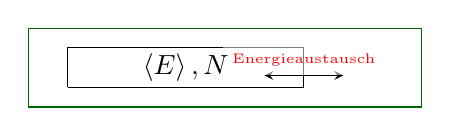
\begin{tikzpicture}[scale=0.5]
    \draw[green!40!black] (0,0)--(10,0)--(10,2)--(0,2)--(0,0);
    \draw (1,0.5)--(7,0.5)--(7,1.5)--(1,1.5)--(1,0.5);
    \draw[stealth-stealth] (6,0.8)--(8,0.8) node[above,midway, red, fill=white,opacity=.5,text opacity=1] {\tiny{Energieaustausch}};
    \draw (4,1) node {$\langle E\rangle \, ,N$};
\end{tikzpicture}
\end{center}
\end{wrapfigure}

Das kanonische Ensemble wurde hier mit dem postulierten Prinzip der maximalen Entropie eingeführt.
Die Herleitung kann auch ?rigoroser? erfolgen:\\
Das Gesamtsystem (inkl. Umgebung) kann mittels des mikrokanonischen Ensembles beschrieben werden, das es ein isoliertes System ist.
\\ Will man nun die WS eines Zustands im kleineren Teilsystems wissen, muss man sich folgendes überlegen:\\
Geht im Teilsystem ein Zustand in einen anderen Zustand über, ändert sich die Energie. Es kommt zum Austauschh mit der Umgebung.
\begin{itemize}
    \item Wird die Energie im Teilsystem größer, so muss sie in der Umgebung kleiner werden. Also hat die Umgebung eine hohe Zustandsdichte.
    \item Wird die Energie im Teilsystem kleiner, so wird die Energie in der Umgebung größer. Die Umgebung hat dann eine geringe Zustandsdichte.
\end{itemize}
Indem man die Anzahl an möglichen Zuständen in der Umgebung betrachtet, damit der eben beschreibene \enquote{ Energiefluss} passieren kann, können die selben Beziehungen für das kanonische Ensemble hergeleitet werden.
Damit wird das Prinzip der maximalen Entropie bestätigt.
\color{black}


\subsection{Großkanonisches Ensemble}\label{sec.Großkanonisches Ensemble}

\begin{center}
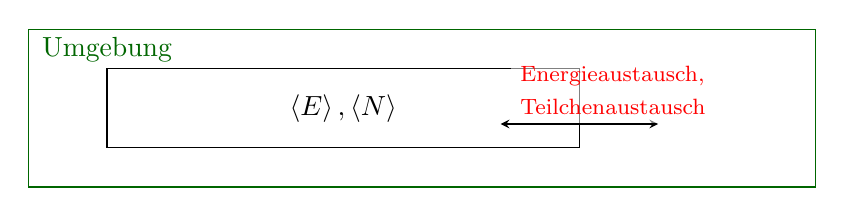
\begin{tikzpicture}
    \draw[green!40!black] (0,0)--(10,0)--(10,2)--(0,2)--(0,0);
    \draw (1,0.5)--(7,0.5)--(7,1.5)--(1,1.5)--(1,0.5);
    \draw[stealth-stealth] (6,0.8)--(8,0.8) node[above, red, fill=white,opacity=.5,text opacity=1, text width=3.5cm] {\footnotesize{Energieaustausch, \\Teilchenaustausch}};
    \draw (4,1) node {$\langle E\rangle \, , \langle N\rangle$};
    \draw (1,1.75) node[green!40!black] {Umgebung};
\end{tikzpicture}
\end{center}

Beispiele:
\begin{itemize}
    \item durchlässige Membran
    \item Elektronentransport
    \item Photonen im Hohlraum
    \item Adsorption
\end{itemize}


\textbf{Ziel:} Dichteoperator $\hat{\varrho}$ bzw. WS $p_n$ für Eigenzustand des Hamiltonoperators mit Energie $E_n$ und Teilchenzahl $N_n$.
\vspace{0.5cm}


Spezialfall: 
\begin{alignat}{2}
    A_1 &= \hat{H} \qquad \lambda_1 &&\rightarrow \beta \\
    A_2 &= \hat{N} \qquad \lambda_2 &&\rightarrow \alpha = - \beta \mu
\end{alignat}
mit $\hat{N}$ - Teilchenzahloperator und $\mu$ chemisches Potential (Eigenschaft der Umgebung)

\begin{equation}
    \fcolorbox{red}{white}{$\varrho_G = \frac{1}{Z} e^{-\beta H - \alpha N}$}
\end{equation}
\begin{equation}
    \fcolorbox{red}{white}{$Z_G(\beta,\alpha) = \trace(e^{-\beta H - \alpha N})$} = \trace(e^{- \beta (H-\mu N)})
\end{equation}
In der Basis der Eigenzustände $\{\ket{\phi_n}\}$:
\begin{equation}
    \fcolorbox{black}{white}{$p_n = \frac{1}{Z_G} e^{-\beta E_n - \alpha N_n}$} \qquad \fcolorbox{black}{white}{$Z_G(\beta, \alpha) = \sum_n e^{- \beta E_n - \alpha N_n}$} 
\end{equation}
Erwartungswerte:
\begin{equation}
    \langle N \rangle = - \frac{\partial}{\partial \alpha} \ln(Z_G(\beta,\alpha)) \quad , \quad \langle E \rangle = - \frac{\partial}{\partial \beta} \ln(Z_G(\beta,\alpha))
\end{equation}
Entropie:
\begin{align}
    S(\langle E \rangle,\langle N \rangle) &= k \ln(Z_G(\beta,\alpha)) + k \beta \langle E \rangle + k \alpha \langle N \rangle \\
    \frac{\partial S}{\partial \langle N \rangle} &= k \alpha = - k \beta \mu \color{black!50!white} = - \frac{\mu}{T} \color{black} \\
    \frac{\partial S}{\partial \langle E \rangle} &= k \beta \color{black!50!white} = \frac{1}{T} \color{black}
\end{align}



\begin{center}
    \begin{tikzpicture}
        \draw[->, line width=1.5pt] (-0.01,0) -- (5.2,0) node[right] {};
  \draw[->, line width=1.5pt] (0,-0.5) -- (0,3.5) node[above] {$E$};
  \draw[] (0,1)--(2.5,1){};
  \draw[] (0,1.5)--(2.5,1.5){};
  \draw[] (0,2)--(2.5,2){};
  \draw[] (0,3)--(2.5,3){};
  \draw[pattern=north west lines, pattern color=blue!50!white] (3,1.5) rectangle (6,2.2) ;
  \node[text width =3cm] at (6,1.75){$\mu$};
  \node[text width =3.5cm, right, blue] at (6,1.7) {\footnotesize{chemisches Potential\\ der Umgebung}};
  \draw[->] (3.2,2.2)  to [out=90,in=90] node[midway,above left,inner sep=2pt, red] {\tiny{Energiezufuhr}} (1,1);
  \draw[<-] (3.5,2.2)  to [out=90,in=90] node[midway,above right,inner sep=2pt, red] {\tiny{Energieabgabe}} (1,3);
    \end{tikzpicture}
\end{center}

\subsection{Fundamentale Fragen} \marginpar{VL. 10}
 \subsubsection{Gibbsches Paradoxon}

 
\begin{center}
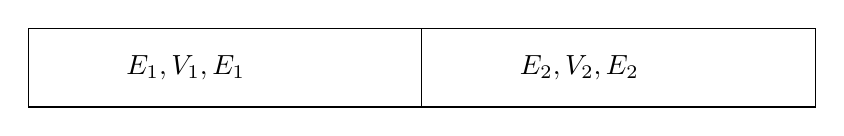
\begin{tikzpicture}
    \draw[black] (0,0)--(5,0)--(5,1)--(0,1)--(0,0);
    \draw (5,0)--(10,0)--(10,1)--(0,1);
    \draw (2,0.5) node {$E_1, V_1, E_1$};
    \draw (7,0.5) node {$E_2, V_2, E_2$};
\end{tikzpicture}
\end{center}

Zwei ideale Gase, gleiche Dichte $\frac{N_1}{V_1} = \frac{N_2}{V_2}$, im Mittel gleiche Energie pro Teilchen $\frac{E_1}{N_1} =\frac{E_2}{N_2}$, gleiche Massen $m_1=m_2$

\textbf{Frage:} Entropieänderung bei Herausnehmen der Wand?

\textbf{ideales Gas} (mikrokanonisch, klassisch, Kap. \ref{seq.Mikrokanonisches_ensemble}) ununterscheidbare Teilchen, d.h. ohne Faktor $\frac{1}{N!}$.
\begin{equation}
    M(E)= \frac{\int_{H(\Vec{q}, \Vec{p}) \leq E} d\Vec{p} d\Vec{q}}{h^{3N}} = \stackrel{\ref{seq.ideales Gas}}{...} = \stackrel{\text{Übung 7.2}}{...} = \left(\frac{V}{\lambda^3} e^{3/2}\right)^N
\end{equation}
mit \begin{equation}
    \lambda = \frac{h}{\sqrt{\frac{4}{3}} \pi m \frac{E}{N}}
\end{equation}

\color{black!50!white}
\paragraph{Bemerkung} für kanonisches Enseble mit $E= 3N \frac{1}{2} k T$ folgt:
\begin{equation}
    \fcolorbox{red}{white}{$\lambda = \frac{h}{\sqrt{2 \pi mkT}} \hspace{2cm} \text{thermische De-Broglie Wellenlänge}$}
\end{equation}

Nenner $\propto $ Impuls bei $kT$.
\color{black}

Entropie:
\begin{equation}\label{eq:Entropie_Gibsses Paradoxon}
    S(N,V,E) = k \ln{(M_{\Delta}(E))} \approx k \ln{(M(E))} = kN \left( \ln \left( \frac{V}{\lambda^3}\right) + \frac{3}{2}\right)
\end{equation}


\textbf{Erwartungen:}
\begin{itemize}
    \item[] $S_{\footnotesize{\textit{ohne Wand}}}^{\footnotesize{\textit{verschiedene Teilchen}}} > S_{\footnotesize{\textit{Wand}}}$  (, da ohne Wand größerer Mangel an Information)
    \item[] 
    \item[] $S_{\footnotesize{\textit{ohne Wand}}}^{\footnotesize{\textit{identische Teilchen}}} = S_{\footnotesize{\textit{Wand}}}$ (, da eigentlich keine Information gewonnen oder verloren wird)
\end{itemize}


\textbf{mit Wand:}
\begin{align}
    S_{\footnotesize{\textit{Wand}}} &= S(N_1,V_1,E_1) + S(N_2,V_2,E_2) \\&\stackrel{(\ref{eq:Entropie_Gibsses Paradoxon})}{=} k N_1 \ln\left(\frac{V_1}{\lambda^3}\right) + k N_2 \ln\left(\frac{V_2}{\lambda^3}\right) +k (N_1+N_2)^\frac{3}{2}
\end{align}

\textbf{ohne Wand, verschiedene Teilchen:}
\begin{align}
    S_{\footnotesize{\textit{ohne Wand}}}^{\footnotesize{\textit{verschiedene Teilchen}}} &= S(N_1,V_1+V_2,E_1) + S(N_2,V_1+V_2,E_2) \\&\stackrel{(\ref{eq:Entropie_Gibsses Paradoxon})}{=} k N_1 \ln\left(\frac{V_1+V_2}{\lambda^3}\right) + k N_2 \ln\left(\frac{V_1+V_2}{\lambda^3}\right) +k (N_1+N_2)^\frac{3}{2}\\
    &> S_{\footnotesize{\textit{Wand}}} \hspace{1cm} \Rightarrow \ \text{1. Erwartung bestätigt}
\end{align}

\textbf{ohne Wand, identische Teilchen:}
\begin{align}
    S_{\footnotesize{\textit{ohne Wand}}}^{\footnotesize{\textit{identische Teilchen}}} &= S(N_1+N_2,V_1+V_2,E_1+E_2)  \\&\stackrel{(\ref{eq:Entropie_Gibsses Paradoxon})}{=} k (N_1 +N_2)\ln\left(\frac{V_1+V_2}{\lambda^3}\right) +k (N_1+N_2)^\frac{3}{2} \\
    &= S_{\footnotesize{\textit{ohne Wand}}}^{\footnotesize{\textit{verschiedene Teilchen}}}\\
    &> S_{\footnotesize{\textit{Wand}}} \hspace{1cm} \Rightarrow \ \text{\Lightning Widerspruch zur 2. Erwartung}
\end{align}


\textbf{Lösung:}
Klassisch müssen wir in QM, identische Teilchen als ununterscheidbar angesehen werden.\footnote{Vorher: Naiv wurde angenommen, dass klassisch Teilchen unterschiedbar sein müssen. D.h., dass man im Phasenraum die Trajektorien aller Teilchen uneingeschränkt nachverfolgen kann. \\
Jetzt: Tatsächlich sind auch klassisch identische Teilchen nicht unterscheidbar.\\
In der QM werden Teilchen als Wellenpacket angenommen. Wenn diese sich vermischen bzw. ineinander laufen, sind diese danach ebenfalls nicht zu unterscheiden.}
\begin{itemize}
    \item[$\Rightarrow$] Permutation identischer Teilchen liefter keinen neuen Zustand
    \item[$\Rightarrow$] Faktor $\frac{1}{N!}$ bei Zahl der Zustände
    \item[$\Rightarrow$] \textbf{korrekte Formel für ideales Gas}
\end{itemize}
\begin{align}
    M(E) &= \frac{1}{N!} \ \frac{\int_{H(\Vec{q}, \Vec{p})<E} d\Vec{p}\, d\Vec{q}}{h^{3N}} \stackrel{\text{Stirling}}{\approx} \left( \frac{V}{N \lambda^3} e^{\frac{5}{2}} \right) ^N\\
    S&= k N \left( \ln\left(\frac{V}{N \lambda^3}\right) + \frac{5}{2}\right)
\end{align}

Löst Gibbsches Paradoxon (siehe Ü 7.2)






\subsubsection{Poincaré-Rückkehr Theorem}

\begin{definition}{Poincaré-Rückkehr Theorem}
    \textbf{Vorraussetzungen:}\\
    Hamiltonsystem mit \underline{endlichen} Phasenraumvolumen bei $H(\Vec{q}, \Vec{p}) = E$.

    \begin{tcolorbox}[colback=red!10!white,colframe=red!10!white]
    Phasenraumpunkte, die ein Phasenraumgebiet $\Gamma_0$ verlassen, kommen irgendwann (fast alle) wieder zurück nach $\Gamma_0$. \\
    Außnahmen, die nicht zurück kommen, haben Volumen Null.
    \end{tcolorbox}
\end{definition}

\begin{center}
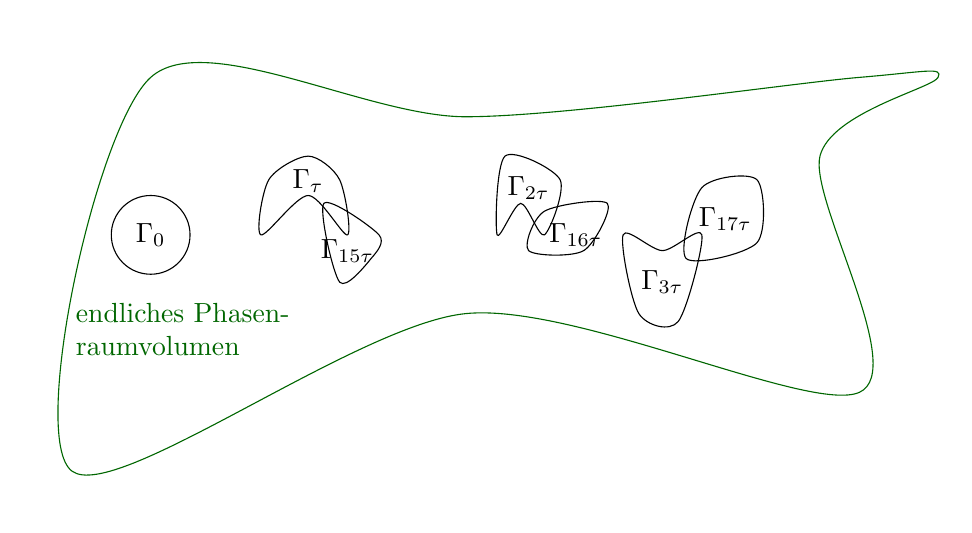
\begin{tikzpicture}
 \draw [green!40!black] plot [smooth cycle] coordinates {(0,0) (5,2) (10,1) (9.5,4) (11,5) (10,5) (5,4.5)  (1,5)};
    \draw (1.8,1.8) node[green!40!black, text width=3.5cm] {endliches Phasenraumvolumen};
    \draw (1,3) circle[radius = 0.5] node {$\Gamma_0$}; 
    \draw plot [smooth cycle] coordinates {(2.4,3) (3,3.5) (3.5,3) (3.4,3.7) (3,4) (2.5,3.7)} node at (3,3.68) {$\Gamma_{\tau}$};
    \draw plot [smooth cycle] coordinates {(3.4,2.4) (3.8,2.7)  (3.9,3) (3.2,3.4)} node at (3.5,2.8) {$\Gamma_{15\tau}$};
    \draw plot [smooth cycle] coordinates {(5.4,3) (5.7,3.4) (6,3) (6.2,3.7)  (5.5,4)} node at (5.8,3.6) {$\Gamma_{2\tau}$};
      \draw plot [smooth cycle] coordinates {(6,3.3) (6.8,3.4) (6.5,2.8) (5.8,2.8)  } node at (6.4,3) {$\Gamma_{16\tau}$};
    \draw plot [smooth cycle] coordinates {(7.2,2) (7.7,1.9) (8,3) (7.5,2.8) (7,3)} node at (7.5,2.4) {$\Gamma_{3\tau}$};
    \draw plot [smooth cycle] coordinates {(7.8,2.7) (8.7,2.9) (8.7,3.7) (8,3.6) } node at (8.3,3.2) {$\Gamma_{17\tau}$};
\end{tikzpicture}
\end{center}

\begin{proof}{Lemma: \textit{ mindestens ein Teilvolumen kehrt zurück.}}\label{Lemma_poincare}\\
    Annahme: Zur Zeit $\tau$ gelte für zeitentwickeltes Gebiet $\Gamma_{\tau}: \hspace{1cm}\Gamma_{\tau} \cap \Gamma_0 = \emptyset $.\\
    Nach \textbf{Lioville Therorem} sind die Volumina $\Gamma_0, \Gamma_{\tau}, \Gamma_{2\tau}, ...$ gleich groß. Das erreichbare Phasenraumvolumen ist allerdings endlich.
\begin{align*}
    \Rightarrow & \exists m,n : & &\Gamma_{m \tau} \cap \Gamma_{n\tau} &\text{ hat Volumen > 0} \\
     \Rightarrow &  & &\Gamma_{(m-1 )\tau} \cap \Gamma_{(n-1)\tau} &\text{ hat Volumen > 0} \\
     \Rightarrow& ... &&&\\
      \Rightarrow &  & &\Gamma_{(m-n) \tau} \cap \Gamma:{0} &\text{ hat Volumen > 0} \\
\end{align*}
$\Rightarrow$ Ein Teil von $\Gamma_0$ mit Volumen >0 ist nach Zeit $(m-n) \tau$ zurückgekommen
\end{proof}
\begin{proof}{Poincaré-Rückkehr Theorem durch Widerspruch}
    Angenommen, es gäbe ein Volumen >0, das nicht zu $\Gamma_0$ zurückkommt $\stackrel{\textit{Lemma}}{\Rightarrow}$ Teilvolumen davon kommt zu $\Gamma_0$ zurück. \Lightning
\end{proof}

\textbf{Bemerkung:}
\begin{itemize}
    \item Macht keine Aussage für einzelne Phasenraumpunkte (einzelner Phasenraumpunkt kommt ggf. nie zurück) \footnote{Beachte: In einem $N$-dimensionalen Phasenraum bildet eine $N-1$-dimensionale Hyperfläche nach dem hier verwendeten Lebesquemaß eine Nullmenge.}
    \item Verteilung der Rückkehrzeit ?
    \item hat für hohe Dimensionen (z.B. $10^2^3$) keine praktische Relevanz
\end{itemize}

\begin{beispiel}{Pendel}
        \begin{center}
        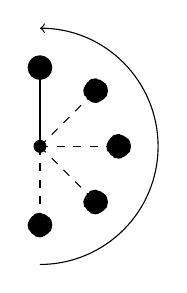
\begin{tikzpicture}
            \draw (0,0) node [circle, draw = black, fill = black,inner sep=1.5pt] {};
            \draw[dashed] (0,0) --(0,-1) node (0,-1) [circle, draw = black, fill = black,inner sep=3pt] {};
            \draw[dashed] (0,0) --(0.707,-0.707) node ((0.707,-0.707) [circle, draw = black, fill = black,inner sep=3pt] {};
            \draw[dashed] (0,0) --(1,0) node (1,0) [circle, draw = black, fill = black,inner sep=3pt] {};
            \draw[dashed] (0,0) --(0.707,0.707) node ((0.707,0.707) [circle, draw = black, fill = black,inner sep=3pt] {};
            \draw (0,0) --(0,1) node (0,1) [circle, draw = black, fill = black,inner sep=3pt] {};
            \draw [->](0,-1.5) arc (-90:90:1.5);
        \end{tikzpicture}
    \end{center}

Ein Pendel kann so ausgelenkt werden, dass es im instabilen Gleichgewicht genau oben stehen bleibt. Dieser Phasenraumpunkt wird also nie zurückkehren. Es gibt unendlich viele Phasenraumpunkte dieses Pendels (von einem bestimmten Ort mit der passenden Geschwindigkeit) so auszulenken, sodass es oben stehen bleibt.

Diese Punkte bilden im gesamten Phasenraum allerdings eine Nullmenge.
\end{beispiel}



\subsubsection{Ergodenhypothese} \marginpar{VL 11}
\begin{itemize}
    \item[Problem] klassische Erwartungswerte ergeben sich aus Ensemblemittel (Phasenraummittel)
    \item[Idee]/Hoffnung: Trajektorie durchläuft zeitlich den gesamten Phasenraum gleichmäßig, d.h.
    \begin{align}
        &\text{Phasenraummittel} &= \quad &\text{Zeitmittel} \\
        &\frac{\int \, \varrho(\Vec{q},\Vec{p}) f(\Vec{q},\Vec{p}) \, d\Vec{q}d\Vec{p}}{\int \, \varrho(\Vec{q},\Vec{p}) \, d\Vec{q}d\Vec{p}} & &\lim_{\tau \to \infty} \frac{1}{\tau} \int_0^{\tau} \, f(\Vec{q}(t),\Vec{p}(t)) \, dt
    \end{align}
\end{itemize}
\begin{definition}{Ergodizität}
    $\exists$ WS-Dichte $\varrho(\Vec{q},\Vec{p})$, so dass Phasenraummittel = Zeitmittel für beliebig Observale und für fast alle Trajektorien
    \begin{equation}
        \langle f(\Vec{q},\Vec{p}) \rangle_{\Gamma} = \langle f(\Vec{q}(t),\Vec{p}(t)) \rangle_t
    \end{equation}
\end{definition}

\begin{prop}{Ergodenhypothese}
    Annahme der Ergodizität in makroskopischen Systemen
\end{prop}
Sind hamiltonische Systeme wirklich ergodisch?

\begin{beispiel}{ergodische Systeme}
    \begin{itemize}
    \item System mit 1 Freiheitsgrad:
\begin{center}
    \begin{tikzpicture}
  \draw[->, thick] (-0.01,0) -- (4.2,0) node[right] {$x$};
  \draw[->, thick] (0,-0.5) -- (0,1.5) node[above] {$E$};
  \draw[color=red, <->]   (1.14,0.5)--(3.14,0.5)   node[right] {$E_1$};
  \draw[dashed] (3.14,0) --(3.14,1);
  \draw[dashed] (1.14,0) --(1.14,1);
  \node[below] at (3.14,0) {$L$};
\end{tikzpicture}
\end{center}
    offensichtlich ist Zeitmittel=Phasenraummittel, da $\Vec{p}$ nur von rechts nach links oder umgekehrt zeigen kann und $\abs{\Vec{v}} = const.$.\\
    Damit wird der gesamte Phasenraum durch abgedeckt.
    \item System mit 2 Freiheitsgraden

    \begin{center}
        \begin{tikzpicture}
            \draw (0,2)--(0,0)--(4,0)--(4,2);
            \draw plot [smooth] coordinates{(0,2) (1,2) (2,2.5) (3,2) (4,2)};
        \end{tikzpicture}
    \end{center}
    Es gibt Bereiche (im Phasenraum) mit regulärer Dynamik und Bereiche chaotischer Dynamik $\rightarrow$ nicht ergodisch
    \item man kann immer eine Observable f finden, so dass System \enquote{ergodisch} ist, aber für tatsächliche Ergodizität muss diese Eigenschaft für \textbf{alle} Observablen gelten
    \item i.A. wird angenommen, dass Systeme mit sehr vielen ($~10^{23}$) Freiheitsgraden ergodisch sind, allerdings sind auch Ausnahmen bekannt und das ist nicht bestätigt
    \item Ergodizität kann auch für QM formuliert werden
\end{itemize}
\end{beispiel}

\subsubsection{Irreversibilität}
In der Natur ist eine bestimmte Zeitrichtung natürlicherweise ausgezeichnet: Wir altern usw... Allerdings zeichnet sich ein Hamilton’sches System durch die Invarianz unter Zeitumkehr aus.
\begin{itemize}
    \item Beispiel TUD Logo:
    \begin{itemize}
        \item am Anfang TUD Logo im Billard aus Kugeln
        \begin{center}
            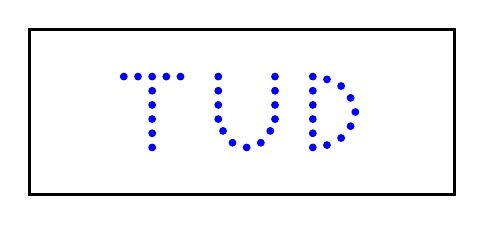
\begin{tikzpicture}[scale=0.60]
                \draw[very thick] (-1,0) rectangle (8,3.5);
                \filldraw[blue] (1,2.5) circle (2pt);
                \filldraw[blue] (1.3,2.5) circle (2pt);
                \filldraw[blue] (1.6,2.5) circle (2pt);
                \filldraw[blue] (1.9,2.5) circle (2pt);
                \filldraw[blue] (2.2,2.5) circle (2pt);
                \filldraw[blue] (1.6,2.2) circle (2pt);
                \filldraw[blue] (1.6,1.9) circle (2pt);
                \filldraw[blue] (1.6,1.6) circle (2pt);
                \filldraw[blue] (1.6,1.3) circle (2pt);
                \filldraw[blue] (1.6,1.0) circle (2pt);
                \filldraw[blue] (3,2.5) circle (2pt);
                \filldraw[blue] (3,2.2) circle (2pt);
                \filldraw[blue] (3,1.9) circle (2pt);
                \filldraw[blue] (3,1.6) circle (2pt);
                \filldraw[blue] (3.1,1.35) circle (2pt);
                \filldraw[blue] (3.3,1.1) circle (2pt);
                \filldraw[blue] (3.6,1) circle (2pt);
                \filldraw[blue] (4.2,2.5) circle (2pt);
                \filldraw[blue] (4.2,2.2) circle (2pt);
                \filldraw[blue] (4.2,1.9) circle (2pt);
                \filldraw[blue] (4.2,1.6) circle (2pt);
                \filldraw[blue] (4.1,1.35) circle (2pt);
                \filldraw[blue] (3.9,1.1) circle (2pt);
                \filldraw[blue] (5,2.2) circle (2pt);
                \filldraw[blue] (5,2.5) circle (2pt);
                \filldraw[blue] (5,1.9) circle (2pt);
                \filldraw[blue] (5,1.6) circle (2pt);
                \filldraw[blue] (5,1.3) circle (2pt);
                \filldraw[blue] (5,1.0) circle (2pt);
                \filldraw[blue] (5.3,2.44) circle (2pt);
                \filldraw[blue] (5.6,2.3) circle (2pt);
                \filldraw[blue] (5.8,2.05) circle (2pt);
                \filldraw[blue] (5.9,1.75) circle (2pt);
                \filldraw[blue] (5.8,1.45) circle (2pt);
                \filldraw[blue] (5.6,1.2) circle (2pt);
                \filldraw[blue] (5.3,1.05) circle (2pt);
            \end{tikzpicture}
        \end{center}
        \item Start der Kugeln mit zufälligen Anfangsbedingungen
        \item nach gewisser Zeit Zeitumkehr
        \item[$\Rightarrow$] je nach Zeitpunkt TUD Logo gut bis gar nicht zu erkennen
        \item[$\rightarow$] chaotisches System, Abweichungen durch Potenzierung der Ungenauigkeiten durch endliche Genauigkeit bei der Rechnung 
    \end{itemize}
\end{itemize}

\subsubsection{Maxwell Dämon}
\begin{itemize}
    \item System mit getrennten Kammern, Trennung: Tür die nur von einer Seite durchlässig ist (Dämon öffnet und schließt die Tür je nachdem von wo das Teilchen kommt)
    \item nach gewisser Zeit ist Druck auf der einen Seite höher
    \item[$\Rightarrow$] Druckausgleich zur Energiegewinnung
    \item[$\Rightarrow$] Perpetuum mobile 
\begin{table}[h]
    \centering
    \begin{tabular}{c|c}
        Variante 1 & Variante 2 \\ \hline
        Gas homogen verteilt & Gas homogen verteilt \\
        A $\rightarrow$ B $\Rightarrow$ Tür offen & A $\rightarrow$ B, wenn $v > v_0$ \\
        B $\rightarrow$ A $\Rightarrow$ Tür zu & B $\rightarrow$ A, wenn $v \leq v_0$ \\
        $\stackrel{\text{Zeit}}{\Rightarrow}$ mehr Teilchen in B & $\stackrel{\text{Zeit}}{\Rightarrow}$ langsame Teilchen in A, T klein \\
        $\Rightarrow$ Energiegewinnung durch Druckausgleich & $\Rightarrow$ schnelle Teilchen in B, T groß
    \end{tabular}
    \label{tab:Maxwell Dämon}
\end{table}
    \item[$\Rightarrow$] Heizung / Energiegewinnung
\end{itemize}

$\rightarrow$ Problem: Tür auf molekularer Ebene bauen

\subsubsection{Feynman-Ratsche}
\begin{itemize}
    \item[] Nutzung einer Ratsche (nur Bewegung in eine Richtung möglich). Damit stellt sich die Frage: Kann man aus der thermischen Bewegung eine gerichtete Bewegung erzeugen?
    \item[]
    \item[] Problem: auch das Ratschen-Blatt fluktuiert thermisch, sodass Ratsche auch zurück kann
    \item[]
    \item[] \textbf{Im Allgemeinen:} Das sind Gedankenexperimente, die (noch) nicht realisert werden konnten und die auch sehr schwer zu realisieren scheinen, allerdings ist nicht bewiesen wurden, dass sie nicht funktionieren.
\end{itemize}




